\documentclass{article}
\usepackage{xeCJK}
\usepackage{fontspec}
\usepackage{listings}
\usepackage{xcolor}
\usepackage{amsmath}
\usepackage{graphicx}
\usepackage{geometry}

\geometry{papersize={182mm , 257mm}}
\geometry{left=1.5cm,right=1.5cm,top=1.5cm,bottom=2.0cm}

\setCJKmainfont{方正楷体_GBK}
\XeTeXinputencoding "UTF-8"


\title{$\text{\Huge{{\setmainfont{UnPilgi} SingleDog}}}_{\text{\setmainfont{UnPilgi} V1.0}}$}
\author{$\text{\setmainfont{UnPilgi} Wumpus GYH}$}
\date{2015.8}

\begin{document}
%Settings

\lstset{
numbers=left,
showspaces=false,
showstringspaces=false,
basicstyle=\ttfamily,
keywordstyle=\bfseries\color{purple!80},
commentstyle=\color{red!50!green!50!blue!50},
rulesepcolor=\color{red!20!green!20!blue!20},
stringstyle=\color{orange},
tabsize=4,
language=C++,
escapeinside=``,
xleftmargin=2em,
xrightmargin=2em,
aboveskip=1em
}

% % % % % % % % % % % % % % % % % % % % % %
%Face
\begin{titlepage}

\maketitle
\setcounter{page}{0}
\thispagestyle{empty}

\begin{verbatim}

                       ::
                      :;J7, :,                        ::;7:
                      ,ivYi, ,                       ;LLLFS:
                      :iv7Yi                       :7ri;j5PL
                     ,:ivYLvr                    ,ivrrirrY2X,
                     :;r@Wwz.7r:                :ivu@kexianli.
                    :iL7::,:::iiirii:ii;::::,,irvF7rvvLujL7ur
                   ri::,:,::i:iiiiiii:i:irrv177JX7rYXqZEkvv17
                ;i:, , ::::iirrririi:i:::iiir2XXvii;L8OGJr71i
              :,, ,,:   ,::ir@mingyi.irii:i:::j1jri7ZBOS7ivv,
                 ,::,    ::rv77iiiriii:iii:i::,rvLq@huhao.Li
             ,,      ,, ,:ir7ir::,:::i;ir:::i:i::rSGGYri712:
           :::  ,v7r:: ::rrv77:, ,, ,:i7rrii:::::, ir7ri7Lri
          ,     2OBBOi,iiir;r::        ,irriiii::,, ,iv7Luur:
        ,,     i78MBBi,:,:::,:,  :7FSL: ,iriii:::i::,,:rLqXv::
        :      iuMMP: :,:::,:ii;2GY7OBB0viiii:i:iii:i:::iJqL;::
       ,     ::::i   ,,,,, ::LuBBu BBBBBErii:i:i:i:i:i:i:r77ii
      ,       :       , ,,:::rruBZ1MBBqi, :,,,:::,::::::iiriri:
     ,               ,,,,::::i:  @arqiao.       ,:,, ,:::ii;i7:
    :,       rjujLYLi   ,,:::::,:::::::::,,   ,:i,:,,,,,::i:iii
    ::      BBBBBBBBB0,    ,,::: , ,:::::: ,      ,,,, ,,:::::::
    i,  ,  ,8BMMBBBBBBi     ,,:,,     ,,, , ,   , , , :,::ii::i::
    :      iZMOMOMBBM2::::::::::,,,,     ,,,,,,:,,,::::i:irr:i:::,
    i   ,,:;u0MBMOG1L:::i::::::  ,,,::,   ,,, ::::::i:i:iirii:i:i:
    :    ,iuUuuXUkFu7i:iii:i:::, :,:,: ::::::::i:i:::::iirr7iiri::
    :     :rk@Yizero.i:::::, ,:ii:::::::i:::::i::,::::iirrriiiri::,
     :      5BMBBBBBBSr:,::rv2kuii:::iii::,:i:,, , ,,:,:i@petermu.,
          , :r50EZ8MBBBBGOBBBZP7::::i::,:::::,: :,:,::i;rrririiii::
              :jujYY7LS0ujJL7r::,::i::,::::::::::::::iirirrrrrrr:ii:
           ,:  :@kevensun.:,:,,,::::i:i:::::,,::::::iir;ii;7v77;ii;i,
           ,,,     ,,:,::::::i:iiiii:i::::,, ::::iiiir@xingjief.r;7:i,
        , , ,,,:,,::::::::iiiiiiiiii:,:,:::::::::iiir;ri7vL77rrirri::
         :,, , ::::::::i:::i:::i:i::,,,,,:,::i:i:::iir;@Secbone.ii:::
\end{verbatim}
\end{titlepage}
\newpage

% % % % % % % % % % % % % % % % % % % % % %
%Cotents


\tableofcontents

\newpage

% % % % % % % % % % % % % % % % % % % % % %
\section{数学}
\subsection{基础}
\lstinputlisting{../数学/基础.cpp}
\subsection{组合数}
\lstinputlisting{../数学/组合数.cpp}
\subsection{素数}
\lstinputlisting{../数学/素数.cpp}
\subsection{矩阵}
\lstinputlisting{../数学/矩阵.cpp}
\subsection{博弈}
\lstinputlisting{../数学/博弈.cpp}
\subsection{数值}
\lstinputlisting{../数学/数值.cpp}
\subsection{FFT}
\lstinputlisting{../数学/FFT.cpp}
\subsection{方程组}
\lstinputlisting{../数学/方程组.cpp}
% % % % % % % % % % % % % % % % % % % % % %
\section{数据结构}
\subsection{RMQ and 树状数组}
\lstinputlisting{../数据结构/RMQ_树状数组.cpp}
\subsection{分块暴力}
\lstinputlisting{../数据结构/分块暴力.cpp}
\subsection{莫队}
\lstinputlisting{../数据结构/莫队.cpp}
\subsection{CDQ}
\lstinputlisting{../数据结构/CDQ.cpp}
\subsection{树的重心}
\lstinputlisting{../数据结构/树的重心.cpp}
\subsection{树上最远路径}
\lstinputlisting{../数据结构/树上最远路径.cpp}
\subsection{树链剖分}
\lstinputlisting{../数据结构/树链剖分.cpp}
\subsection{平衡树}
\subsubsection{Treap}
\lstinputlisting{../数据结构/treap.cpp}
\subsubsection{SBT}
\lstinputlisting{../数据结构/sbt.cpp}
\subsubsection{Splay}
\lstinputlisting{../数据结构/splay.cpp}
\subsubsection{主席树}
\lstinputlisting{../数据结构/主席树.cpp}
\subsection{LCT}
\lstinputlisting{../数据结构/LCT.cpp}
\subsection{线段树}
\subsubsection{区间Add}
\lstinputlisting{../数据结构/线段树_区间add.cpp}
\subsubsection{非常见线段树}
\lstinputlisting{../数据结构/非常见线段树.cpp}

% % % % % % % % % % % % % % % % % % % % % %
\section{图论}
\subsection{拓扑排序}
\lstinputlisting{../图论/拓扑排序.cpp}
\subsection{最短路}
\lstinputlisting{../图论/最短路.cpp}
\subsection{欧拉回路}
\lstinputlisting{../图论/欧拉回路.cpp}
\subsection{哈密顿}
\lstinputlisting{../图论/哈密顿.cpp}
\subsection{Prim}
\lstinputlisting{../图论/Prim(临时).cpp}
\subsection{二分图}
\lstinputlisting{../图论/二分图.cpp}
\subsection{2SAT}
\lstinputlisting{../图论/2SAT.cpp}
\subsection{LCA}
\lstinputlisting{../图论/LCA.cpp}
\subsection{割点与桥}
\lstinputlisting{../图论/割点与桥.cpp}
\subsection{有向图强连通分量}
\lstinputlisting{../图论/有向图强连通分量.cpp}
\subsection{无向图点双连通分量}
\lstinputlisting{../图论/无向图点双连通分量.cpp}
\subsection{无向图边双连通分量}
\lstinputlisting{../图论/无向图边双连通分量.cpp}
\subsection{网络流}
\lstinputlisting{../图论/网络流.cpp}
\subsection{最小树形图}
\lstinputlisting{../图论/最小树形图.cpp}
\subsection{无向图全局最小割}
\lstinputlisting{../图论/无向图全局最小割.cpp}
% % % % % % % % % % % % % % % % % % % % % %
\section{计算几何}
\subsection{二维}
\lstinputlisting{../计算几何/二维.cpp}
\subsection{三维}
\lstinputlisting{../计算几何/三维.cpp}
% % % % % % % % % % % % % % % % % % % % % %
\section{字符串}
\subsection{KMP}
\lstinputlisting{../字符串/KMP.cpp}
\subsection{manacher}
\lstinputlisting{../字符串/manacher.cpp}
\subsection{Trie}
\lstinputlisting{../字符串/Trie.cpp}
\subsection{Hash}
\lstinputlisting{../字符串/hash.cpp}
\subsection{后缀数组}
\lstinputlisting{../字符串/后缀数组.cpp}
\subsection{AC自动机}
\lstinputlisting{../字符串/AC自动机.cpp}
\subsection{SAM}
\lstinputlisting{../字符串/后缀自动机.cpp}


% % % % % % % % % % % % % % % % % % % % % %
\section{DP}
\subsection{序列DP}
\subsubsection{最长上升子序列}
\lstinputlisting{../DP/LIS.cpp}
\subsubsection{最长公共子序列}
$O(mn)$
\lstinputlisting{../DP/LCS.cpp}
$O(mlogn)$	\\
将LCS转化为LIS问题,应用O(nlogn)的LIS算法即可	\\
假设两个序列 s1 = “abcabc” 和 s2 = “acbdcab”\\
记录s1中每个元素在s2中出现的位置,然后降序排列	\\
pos(a) = {5,0}								\\
pos(b) = {6,2}								\\
pos(c) = {4,1}								\\
\\
然后按照s1及pos排出对应的 s3 ={5,0,6,2,4,1,5,0,6,2,4,1}	\\
最后对s3求LIS即为所求答案,LCS为所选数字对应字母序列。			\\

\subsubsection{最长公共上升子序列}
\lstinputlisting{../DP/LCIS.cpp}
\subsubsection{最短公共子序列}
找到一个最短的字串,其子序列包含了所有给定字串	\\
两个
$$ |SCS|=|S1|+|S2|−|LCS| $$
n个
\lstinputlisting{../DP/SCS.cpp}
\subsubsection{回文子序列}
最长
$$
d(i,j)= \begin{cases}
d_{i+1,j-1} + 2  &s[i]=s[j] \\
Max(d_{i+1,j},d_{i,j-1}) &s[i] \ne s[j]
\end{cases}
$$
统计
$$
d_{i,j}=
\begin{cases}
d_{i+1,j} + d_{i,j-1}   &s[i]=s[j] \\
d_{i+1,j} + d+{i,j-1} - d_{i+1,j-1}  &s[i] \ne s[j]
\end{cases}
$$

\subsection{背包DP}
\subsubsection{多重背包}
\lstinputlisting{../DP/多重背包.cpp}
\subsubsection{混合背包}
\lstinputlisting{../DP/混合背包.cpp}

\subsection{数位DP}
\lstinputlisting{../DP/数位DP.cpp}
\subsection{集合DP}
\lstinputlisting{../DP/SCS.cpp}

\subsection{DP优化}
\subsubsection{四边形不等式}
\lstinputlisting{../DP/四边形不等式.cpp}
\subsubsection{决策单调性}
\lstinputlisting{../DP/决策单调.cpp}

% % % % % % % % % % % % % % % % % % % % % %
\section{魔法}
\subsection{位}
\lstinputlisting{../魔法/位魔法.cpp}
\subsection{黑魔法}
\lstinputlisting{../魔法/奇怪的.cpp}

% % % % % % % % % % % % % % % % % % % % % %
\section{被遗弃的角落}
\subsection{Java}
\lstinputlisting[language = java]{../被遗弃的角落/FastIO.java}
\subsection{Bitset}
\lstinputlisting{../被遗弃的角落/bitset.cpp}
\subsection{分数类}
\lstinputlisting{../被遗弃的角落/分数.cpp}
\subsection{日期类}
\lstinputlisting{../被遗弃的角落/日期.cpp}
\subsection{DLX解数独}
\lstinputlisting{../被遗弃的角落/DLX解数独.cpp}
\subsection{大大大的数}
\subsubsection{BigInteger}
\lstinputlisting{../被遗弃的角落/BigInteger.cpp}
\subsubsection{BigDecimal}
\lstinputlisting{../被遗弃的角落/BigDecimal.cpp}
\subsubsection{简易大整数}
\lstinputlisting{../被遗弃的角落/简易大整数.cpp}
% % % % % % % % % % % % % % % % % % % % % %


\section{记不住的}
\subsection{数学结论}
\lstinputlisting{../记不住的/数学结论.cpp}
\subsection{cout精度}
\lstinputlisting{../记不住的/cout精度.cpp}
\subsection{放颜色不同的球}
\lstinputlisting{../记不住的/放颜色不同的球.cpp}
\subsection{暴力枚举n节点树}
\lstinputlisting{../记不住的/枚举树.cpp}
\subsection{每个点最大/小值区间}
\lstinputlisting{../记不住的/求每个数为最大值的范围.cpp}

% % % % % % % % % % % % % % % % % % % % % %

\section{套路}
\subsection{平面点哈曼顿距离}
\lstinputlisting{../套路/一群点的哈曼顿距离.cpp}
\subsection{求和的乘积最小}
\lstinputlisting{../套路/和的乘积最小.cpp}

% % % % % % % % % % % % % % % % % % % % % %



\section{箴言}

\subsection{定理}
\subsubsection{一般}
1. V + F-2 = E 顶点数+面数-2 = 边数

2. Fibonacci O(1)$$\frac{ ( \frac{1+\sqrt{5}}{2} )^n - (\frac{1-\sqrt{5}}{2})^n ) }{ \sqrt{5} }$$

\newpage
\subsection{数论}
1. 因子个数
$$sum=(e1+1)(e2+1)…(em+1)$$
2. 因子和(等比数列二分求和)
$$sum_n=\prod_1^k \sum_0^{e_i}p_i^j$$\\
筛法预处理
$$\begin{cases}
sum_n = n+1  &n为素数    \\
sum_n = (1 + p + p^2 + … + p^e)*sum_m  & n = p^e*m
\end{cases}
$$
3.LCM(1..n)
由lcm的性质,我们可知

$$lcm(1..n) = 2^{e_1} * 3^{e_2} * 5^{e_3} … \;\; e_i \text{为最大的满足} p_i^{e_i} \le n \text{的值}$$

于是我们从小到大枚举k,然后二分求出前i个素数满足pei≤n,可以提前处理出前i个数的前缀积,然后答案乘上这个前缀积。

$$LCM(C_k^0,C_k^1,…,C_k^k) = \frac{LCM(1,2,…,k,k+1)}{k+1}$$
\newpage
\subsection{排列组合}
1. 隔板法	\\
n个元素(每个可选多次)取出k个。	\\
第i个元素选xi个,转化为 x1+x2+…+xn=k的非负整数解,		\\
令xi+1=yi,则转化为y1+y2+…+yn=k+n的正整数解个数。		\\
即在n+k-1个分割线中中取n-1个,答案:
$$C_{n+k-1}^{n-1}=C_{n+k-1}^{k}$$
2. 卡特兰数	\\
1(C0) 1 2 5 14 42 132 429 1430 4862 16796 …	\\
$$\begin{aligned}
&C_{n+1}=C_0C_n+C_1C_{n-1}+…+C_nC_0 \,\, \Rightarrow  \,\, C_{n+1}= \sum_{i=0}^n C_iC_{n-i} \,\, (n \ge 0 \, , \,C_0=1)	\\
&C_{n}=\frac{4n-2}{n+1}C_{n-1}	\\
&C_n=\frac{(2n)!}{(n+1)!n!}
\end{aligned}
$$
\newpage
\subsection{博弈论}

\subsubsection{Bash Game}

n个棋子,每次最多取m个,最少取1个,到最后不能取的人失败。\\
n\%(m+1)==0 则先手必败,否则先手必胜	\\
因为无论先手怎么拿,后手总可以让其变成n\%(m+1)==0的状态,最后n=m+1时必败	\\

\subsubsection{Wythoff Game}

2堆棋子,每次从一堆或两堆取相同数目,最后不能取的人失败。	\\
奇异局势先手必败,否则先手必胜							 \\
判断(ak,bk)是否为奇异局势:							 \\
$$\begin{aligned}
&ak = [\frac{k(1+\sqrt{5})}{2}] &  k \in N \\
&bk = ak + k                    &  k \in N
\end{aligned}
$$
根据(x,y),y-x=k,判断。	\\

\subsubsection{SG函数/定理}

我们这样定义SG游戏:
\begin{itemize}
\item 游戏两人参与,轮流做出决策。且默认为对自己最有利的决策。
\item 当有一人无法做出决策时游戏结束,无法做出决策的人输。
\item 游戏可以在有限步内结束,同一状态不可能多次抵达。
\item 游戏不会出现平局。
\item 任意一个游戏者在某一状态做出的决策集合只与当前状态有关,与游戏者无关。
\end{itemize}

\textbf{SG函数}

对于任意状态x,SG(x)=mex(S)	\\
S是x后继状态的集合,mex(S)表示不在S内的最小非负整数(自然数)	\\
SG(x)=0表示当前局面必败,否则必胜。

SG函数满足如下性质:
\begin{itemize}
\item 对于任意局面x,若SG(x)=0,那么它的任何一个后继局面的SG都不为0
\item 对于任意局面x,若SG(x)≠0,那么它一定有一个一个后继局面的SG为0
\end{itemize}

或者我们换种理解
\begin{itemize}
\item 对于必败状态,所有后继状态都是必胜的
\item 对于必胜状态,至少有一个后继状态是必败的
\end{itemize}


\textbf{SG定理}

总游戏SG函数的值等于所有子游戏的SG函数值的异或和

\subsubsection{Nim Game}

nim游戏规则如下:
\begin{itemize}
\item 桌子上有N堆石子,游戏者轮流取石子
\item 每次从一堆中取出任意数目的石子,但不能不取
\item 取走最后一个石子者获胜
\item 对于每堆SG(x)=x,然后应用SG定理
\end{itemize}

先手必胜当且仅当:
$$\sum SG(x_i) \neq 0$$

\subsubsection{Anti-nim}

Anti-nim游戏规则只有最后一点与nim不同:取走最后一个石子着败,即获胜条件与nim恰好相反

先手必胜当且仅当:
\begin{itemize}
\item 所有堆的石子数目都为1,且$\sum SG = 0$
\item 至少有一堆石子数目大于1,且$\sum SG \neq 0$
\end{itemize}

\textbf{SJ定理}

我们可以将Anti-nim推广到任意SG游戏即Anti-SG游戏。
先手必胜当且仅当:
\begin{itemize}
\item $\sum SG \neq 0$,且存在单一游戏SG函数大于1
\item $\sum SG = 0$,且没有单一游戏SG函数大于1
\end{itemize}

\subsubsection{Multi-SG}

Multi-SG游戏规则如下:
\begin{itemize}
\item 在符合拓扑原则的前提下,一个单一游戏的后继可以为多个单一游戏。
\item 其余规则与SG游戏相同
\end{itemize}

即可以将一堆石子分成多堆。\\
我们仍然可以用SG函数定义局面。

\subsubsection{Every-SG}

Every-SG游戏规则如下:
\begin{itemize}
\item 对于没有结束的单一游戏,游戏者必须对该游戏进行一步决策
\item 其余规则与SG游戏相同
\end{itemize}

我们考虑让我们必胜的游戏尽可能长地玩下去!	\\
通过拓扑关系计算某一状态的SG函数时候,	\\
对于SG为0的点,我们需要知道最快几步进入终止状态。	\\
对于SG不为0的点,我们需要直到最慢几步进入终止状态。	\\
设当前状态为u,后继状态为v,定义函数step(u)为到终止状态的步数		\\
$$
step(u) = \begin{cases}
0              & u \text{为终止状态} \\
max(step(v))+1 & SG(u)>0 \text{且} SG(v)=0 \\
min(step(v))+1 & SG(u)=0
\end{cases}
$$
则先手必胜当且仅当:

单一游戏中最大的step为奇数

\subsubsection{Staircase Nim}

阶梯博弈规则如下:
\begin{itemize}
\item 从左至右有若干堆石子
\item 每次可以从当前堆取若干石子移动到前面一堆上
\item 最后不能移动者败
\end{itemize}

先手必胜当且仅当:

阶梯的所有奇数位置的SG和不为0

因为如果棋子从奇数位拿到了偶数位,相当于将这些棋子移走。\\
从偶数位置移到奇数位,必胜者可以将这些棋子移到下一个偶数位。

\textbf{poi2009 Pebbles(bzoj1115)}

题目意思是有n堆石子,每次可以从一堆移走若干个,但每堆数目要保持从左至右递增,最后不能取的人败 \\
我们对相邻两堆石子进行差分,令b[i] = a[i] - a[i-1];	\\
那么从第i堆移走k个石子即 b[i] -= 1,b[i+1] += 1;	\\
这样就成了阶梯nim模型,对奇数堆的b[i]求异或和即可。	\\

\begin{lstlisting}
#include<cstdio>
#include<cstring>

const int maxn = 1010;
int save[maxn];

int main()
{
    int T,n,x;
    //freopen("test.txt","r",stdin);
    scanf("%d",&T);
    while(T--)
    {
        scanf("%d",&n);
        int ans = 0;
        for(int i=1;i<=n;++i) scanf("%d",save+i);
        for(int i=n;i>1;i-=2) ans ^= (save[i] - save[i-1]);
        if(n&1) ans ^= save[1];
        puts(ans?"TAK":"NIE");
    }
    return 0;
}
\end{lstlisting}

\subsubsection{翻硬币游戏}

翻硬币游戏规则如下:
\begin{itemize}
\item N枚硬币排成一排,编号为1-N。
\item 一枚硬币有正反两种状态,翻一次改变一次。
\item 游戏者根据某些约束翻硬币(如:每次只能翻一或两枚,或者只能翻连续几枚),但是他所翻动的硬币中,最右边只能从正面翻到反面。
\item 谁不能翻谁输
\end{itemize}

局面的SG值为局面中每个正面朝上的棋子单一存在时候的SG值的异或和

我们理解为位,正面为1,反面为0

 $$SG(011001) = SG(01) \text{\^{}} SG(001) \text{\^{}} SG(000001)$$

\subsubsection{树的删边游戏}

规则如下:
\begin{itemize}
\item 给出一颗N个结点的树,其中一个点为树的根节点
\item 轮流删边,删去一条边后,不与根节点相连的部分被移去
\item 无路可走者败
\end{itemize}

叶子结点SG值为0; 中间结点SG值为所有子节点 (SG值+1) 的异或和

\subsubsection{无向图删边游戏}

规则如下:
\begin{itemize}
\item 给定一个无向联通图,取一个点作为图的根。
\item 轮流删边,删去一条边后,不与根节点相连的部分被移去
\item 无路可走者败
\end{itemize}

我们可以对无向图做如下改动:	\\
将图中的任意一个偶环缩成一个新点,任意一个奇环缩成一个新点加一个新边;	\\
所有连到原先环上的边全部改为与新点相连。	\\
这样的改动不会影响图的 SG 值,无向图的删边游戏就成了树的删边游戏。	\\


% % % % % % % % % % % % % % % % % % % % % %
\newpage
\subsection{蒟蒻的小小备忘}
\subsubsection{Tips}
1.对于1,2,3,...n这个序列所生成的前序序列的二叉树,其中序序列(n个节点的二叉树个数)即为1,2,3,4...n进行栈变化后所产生的序列 \\

2.可行性剪枝与最优化剪枝: 可以先初始时定义一种策略,设定其为下界,进行最优化剪枝 \\

3.可以将有向图a->b->c,中的点进行拆分a''->b',b''->c' \\

4.最大完全子图: 子图中两两点之间都有边相连  做法: 建立原图的补图,在补图中取最大独立集 \\

5.可以将01串中1的个数限制转化为不等关系,使用差分约束系统求解 \\ (注意:F[i] <= F[i+1] <= F[i]+1,这个关系不能忽略) \\

6.Set中使用lower\_bound,需要用S.lower\_bound,用lower\_bound(S.begin(),S.end())很慢 \\

7.图论中拆点: 限制容量,限制路径,以及时间分层!!\\

\subsubsection{DP}
\paragraph{1.求存在m个1连续的01串个数\\}
  dp[i][1] = 2*dp[i-1][1] + dp[i-m][0] , dp[i][0] = 2\^n-dp[i][1] (1成功,0失败)\\
\subsubsection{并查集}
\paragraph{1. 获取该连通分量的个数\\}
只需要在2个连通分量merge的时候,使fa[a] = b , sum[b] += sum[a]即可\\
查询x的节点所在连通分量中元素个数,即为 sum[findfa(x)] \\

\paragraph{2. 获取到根节点的距离\\}
首先需要保证每个根节点在成为子节点后不会再成为新的根节点\\
(即: 每次merge时候,要保证新的根节点的权值为0) \\ ,merge过程只需要 fa[a] = b,并且使a的权值变成新的权值.\\
findfa这个过程:\\
\begin{lstlisting}
	int findfa(int x)
	{
		if(x == fa[x]) return x;
		int t = findfa(fa[x]);
		sum[x] += sum(fa[x]);
		return fa[x] = t;
	}
\end{lstlisting}
在下一次查询时,给a的后继节点都加上a的新权值\\

\paragraph{3. 如hdu2818\\}
注意到,每次merge,a的后继节点应该加上b中连通分量的个数,所以需要综合运用1,2 \\

\paragraph{4. 并查集建立虚根\\
HDU 3234\\
将所有确定的点都连通到虚根n上, 点i的权值表示i到root的异或值. \\ merge的时候,//我们保证根节点在一般情况下为0, 当加入节点时 a--x 需要xor res[x]  b -- y需要 xor[y] 并且x -- y需要xor v 那么 a -- b需要xor res[x] xor res[y] xor v ,之后b的后继就可以进行更新\\
HDU2473 \\
对并查集的删除操作(从连通分量中去除该点),通过建立虚根的方式,使用replace 数组 \\ }

\paragraph{5. 并查集解决最小费用\\}
例如Kruskal

\subsubsection{莫比乌斯反演}
\paragraph{1. 常规的求$gcd(x,y) == a, 1 <= x <= n,1 <= y <= m $\\}
令f(i) 为 $gcd(x,y) == i$的个数\\
令g(i) 为 $gcd(x,y) \% i == 0$的个数,那么$g(i) = n/i$; \\
除一下,即求$gcd(x,y) == 1, 1<= x <= n/a, 1 <= y <= m/a$的个数\\
那么就是:\\
\begin{lstlisting}
for(int i = 1;i < =  maxn;i++)
	res += mu[i]*n/i*m/i;
\end{lstlisting}


\paragraph{2. 变种的求$gcd(Ax,Ay) == a$, 在数列中的个数\\}
	令f(i) 为 $gcd(Ax,Ay) == i$的个数 \\
令g(i) 为 $gcd(Ax,Ay) \% i == 0$的个数,那么g(i) = n/i; \\
首先先对数列中数进行处理,求出数列中能把A[i]整除的数的个数cnt[A[i]],这即为g(A[i]) \\
然后类似的 \\
\begin{lstlisting}
	for(int i = a;i <= maxn;i += a)
		res += mu[i/a] * cnt[i]*cnt[i]    //注意这里mu[i/a],类似前一中情况,而后面的cnt[i] 对应前面的n/i
\end{lstlisting}
要用Mobius反演求集合中$gcd(a[i],a[j]) == k$的个数: \\
\begin{lstlisting}
    for(int j = k;j <= maxn;j += k) \\
        res += mu[j/k]*cnt[j]*(cnt[j]-1)/2; \\
\end{lstlisting}
类似求[1,m]中gcd(i,j) == k的个数 \\
这里定义f(k)是gcd(a[i],a[j]) == k的个数 \\
g(k) 是gcd(a[i],a[j])\%k == 0的个数 \\
那么这里的cnt就是[j,maxn]中可以整除j的个数, \\
处理a[i]时候,要将a[i]的每个因子的cnt都+1

\subsubsection{字符串}
\paragraph{1.连续子串中求第k大的串\\ 把所有后缀插入Trie中,然后在Trie上进行dfs}

\subsubsection{图论}
\paragraph{最短路}

\subparagraph{1.K短路问题\\}
首先在终点做一次Dijkstra,然后从起点开始使用a\_star进行扩展\\ (这里g(n)即为走过的路程,f(n)为当前点到终点的最短距离....实际上,可以只使用g(n)进行扩展,即再次Dijkstra )    ---------------------例题 POJ2449
\subparagraph{2.求最短路和次短路\\}
在update时有4中状态,而且在HeapNdoe中要添加一个mode 记录当前是最短路还是次短路,同样done数组也许要添加1维
\begin{lstlisting}
d[e.to][0] > d[u][mode] + e.w  //更新e.to的最短路
d[e,to][0] == d[u][mode] + e.w  //更新e.to最短路状态
d[e.to][1] > d[u][mode] + e.w //更新e.to的次短路
d[e.to][1] == d[u][mode] + e.w //更新e.to的次短路状态
\end{lstlisting}

\subparagraph{3.最优比率正环( 正环一般都转化成负环)\\}
使用0,1规划  设$$ans =  (F[1] + F[2] + F[3] + … F[n] ) / ( W[1] + W[2] + W[3] + … W[n] )$$
转化一下$$( F[1] – ans*W[1]  ) + ( F[2] – ans*W[2]  ) …$$.不难发现,当这个个式子的值 > 0时,ans非最优答案,还有更好的  我们再转化一下$$(  ans*W[1] – F[1] ) +  ( ans*W[2] - F[2] ) … $$
那么当这个式子小于0,时还有更好的, 那么每次我们只需要找到使左边最小值,就可以知道ans是否是最优解(二分求最优解)  所以只需要将边权值转化成 $ans*W[i] – F[i]$ 用bellman-ford判断是否存在负环即可  ---------- POJ3621
% % % % % % % % % % % % % % % % % % %
\paragraph{生成树}
\subparagraph{1.k度最小生成树(POJ1639)\\
先求一个最小生成树(生成加边的过程中,用G添加边)\\
如果满足k度限制,输出\\
否则,fa重置,从root开始分别dfs其子树,对每一个子树中的点的fa,都合并到与root相连的这个儿子上,那么就分离出了和root相连的若干个连通分量.\\
然后,0->m加边(如果可以连通2个连通分量并且端点不是root的话),一直使得为k度\\
最后,0->m加边,构成生成树 \\
自我意淫的做法,这样做的原因: \\ 由于第一次的最小生成树,那么连接这几个连通分量最少的代价就是和root直接相连的边.\\ 此时先合并成了k个,那么这些新添加的边必然没有和root直接相连的边优.所以最后和root相连添加的边必然是原来最小生成树中的}
% % % % % % % % % % % % % % % % %
\paragraph{二分图}
\subparagraph{1.判断二分匹配必须边(POJ1486)\\
先进行二分匹配,然后枚举删除这些匹配边,如果再次dfs失败,那么就是必须边(match[i]需要还原),否则不是(此时match[i]无须还原), 每次枚举结束后还原删除的匹配边can[t][i] = 1;}

\subparagraph{2.各种关系\\
最小点覆盖 = 最大匹配数\\
最小边覆盖= n-最大匹配数 **注意,需要把所有能到达关系都加上---floyed** \\
最小路径覆盖(无环) = 最小边覆盖  \\
最小路径覆盖(有环): \\
(1)i分为i1和i2然后如果i和j有边,那么就在i1和j2之间连一条边。由此构成二分图 然后最小路径覆盖是n-m,n为原图的点的个数,m为新造二分图的最大匹配 \\
(2)强连通分量缩点,变成无环,然后再求
}
% % % % % % % % % % % % % % % % %
\paragraph{图中判环}
\subparagraph{1. 在无向图判环:并查集}
\subparagraph{2. 在有向图判环:拓扑排序(如果不能,就是有环)}
\subparagraph{3. 有向图+无向图: 先并查集判断,如果此时不存咋,就将一个连通分量缩成1个点,再来拓扑排序}
\subparagraph{4. 无向图中是否有奇数环:  非二分图必有奇数环}
\subparagraph{5. 无向图中是否有偶数环: \\ 分离出所有的双连通分量,然后分别检测是否有偶环 \\
(1) 如果是单环,直接判断即可 \\
(2)如果是2个缠绕(贡献至少一条边)的环,如果这2个都是奇数环,那么可以通过去除中间的公共边,使得变成偶数环,所以这种情况必定存在偶数环}
% % % % % % % % % % % % % % % % % % % % % %
\paragraph{点覆盖问题}
\subparagraph{1. 最小点覆盖: 转化为二分图匹配问题}
\subparagraph{2. 点带权求费用最少的覆盖: 定义s,t(超级源和超级汇)  s->x的边权值为x的费用, y->t的边的的权值为y的费用,x->y的权值为INF,问题就转化成最小割(去掉费用和最少的边使得s-t不连通,由于将x->y的边权值定为INF,所以最小割一定不会选取x->y的边,也就是肯定选择s->x或者y->t的边,即选择点),再将最小割转化成求最大流,边权转为边的容量,最大流量即为最小割的结果... 注:POJ3308}
% % % % % % % % % % % % % % % % % % % % % %
\paragraph{网络流}
\subparagraph{1.无源无汇可行流: u--->v 容量为c-b, ST--->v 容量为b, u--->TT 容量为b,求SS--->TT最大流(仅当 $\sum in[i] == D.getRes(SS,TT)$时有解) ,输出时e.cap + down[u][v]}
\subparagraph{2.有源有汇可行流: 在1的基础上增加T---->S 容量为INF}
\subparagraph{3.有源有汇最大流: 在2的基础上求可行流,然后把T---->S边去除(流量置满) 求S---->T最大流即为结果,输出为e.cap + down[u][v]}
\subparagraph{4.有源有汇最小流: 在2的基础上先不加上T---->S,另now1 = D.getRes(SS,TT),然后加上T---->S,另now2 = D.getRes(SS,TT),如果$now1 + now2 != \sum in[i]$,无解,否则结果为T---->S的流量,输出为e.cap + down[u][v]}
\subparagraph{5.最小割输出结果: \\
(1)要输出割集:从S开始dfs,走还剩余容量的边,走到的点vis = 1,最后如果一条边两个端点vis分别为1,0,那么这条边就是割集中的 \\
(2)要输出只改变一边容量使得流量变大的:从S开始dfs一遍,标记,再从T开始dfs一遍,再次标记,一条边的端点分别拥有2种标记的就是所求}
\subparagraph{6.最大密度子图(POJ3155) \\
将图建为: S—>u 容量为U,u—->T 容量为U+2ans-d[u],u—v有边就互相添加容量为1的边,求最小割c[S,T] \\
则E’-V’ans的最大值即为: (U∗n−c[S,T])/2 \\
最后V’中的点,即为从S开始,沿着还有剩余容量的边dfs的点集}
% % % % % % % % % % % % % % % % % % % % % % % %
\paragraph{其他}
\subparagraph{1.混合图判断欧拉回路: \\
判断是否连通,不连通直接输出 \\
将所有的无向边随意定向,和有向边一起,统计下in,out度数,定义D[i] = out[i]-in[i],由欧拉回路定义可知,如果出现D[i]为奇数,必然不存在 \\
下面目标就是将这些随意定向的边选择一些转向.使用网络流模型.\\先把这些随意定向的无向边加入新图中,容量为1,表示最多只能被改变1次.对于所有点来说假设D[a] > 0,那么添加一条S—>a,容量为D[i]/2的边,如果D[b] < 0,那么添加一条边b—>T,容量为-D[i]/2的边. 跑网络流,\\如果从S出发的边都满载,那么只需要把图中不和S,T连接,且流量为1的边转向,即可构成欧拉回路.否则不存在\\
至于为何这样建图,观察到S—>i—>j—>k—>T,这条链上进行转向,那么只有和S,T连接的点i,k的D值会改变.所以,从S出发的边都满载时,所有D不等于0的点的D值才能被改变成0\\
混合图判断欧拉道路\\
必然只存在2点的D为奇数,这两点分别为入点和出点\\
我们手动给这两点加上一条边,然后按照上面判断欧拉回路即可.\\
最后把加的这条边去掉即可\\}
% % % % % % % % % % % % % % % % % % % % % %
\section{附录}
\subsection{Q神尸兄的祖传公式}

\newpage
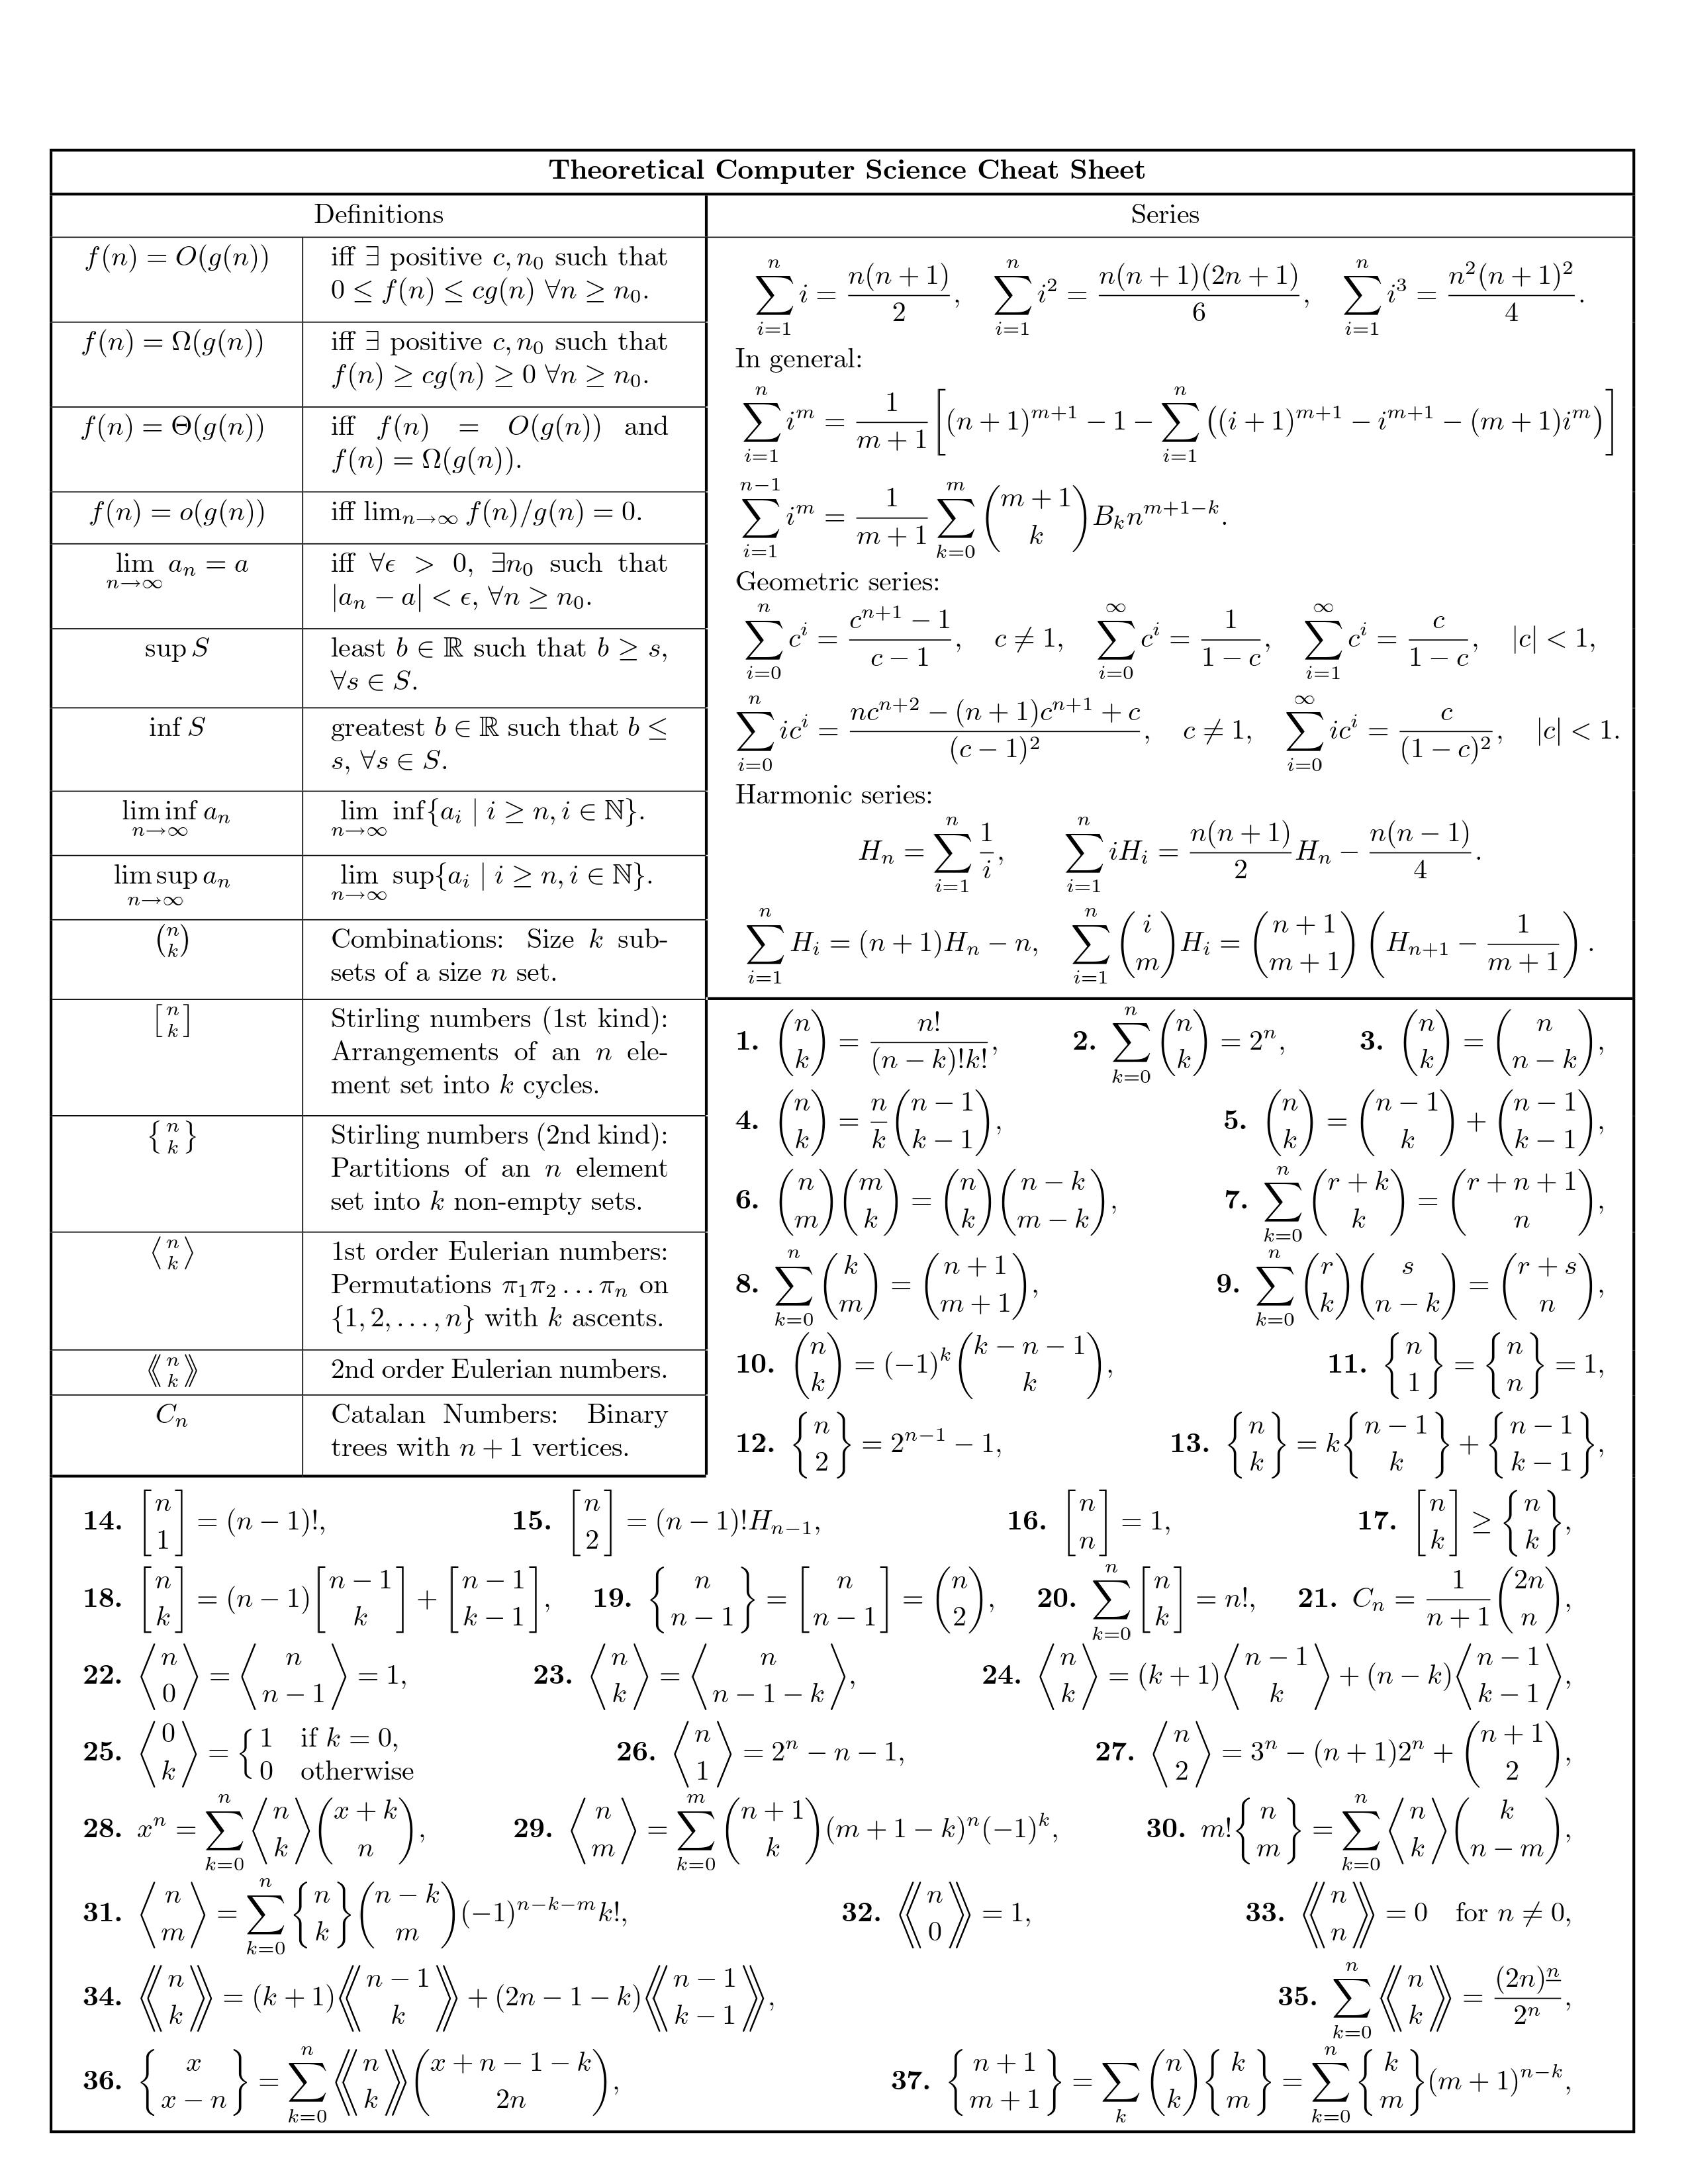
\includegraphics[trim = 6mm 2mm 0mm 10mm,clip=true,scale = 0.73]{./images/image-0001.jpg}
\newpage
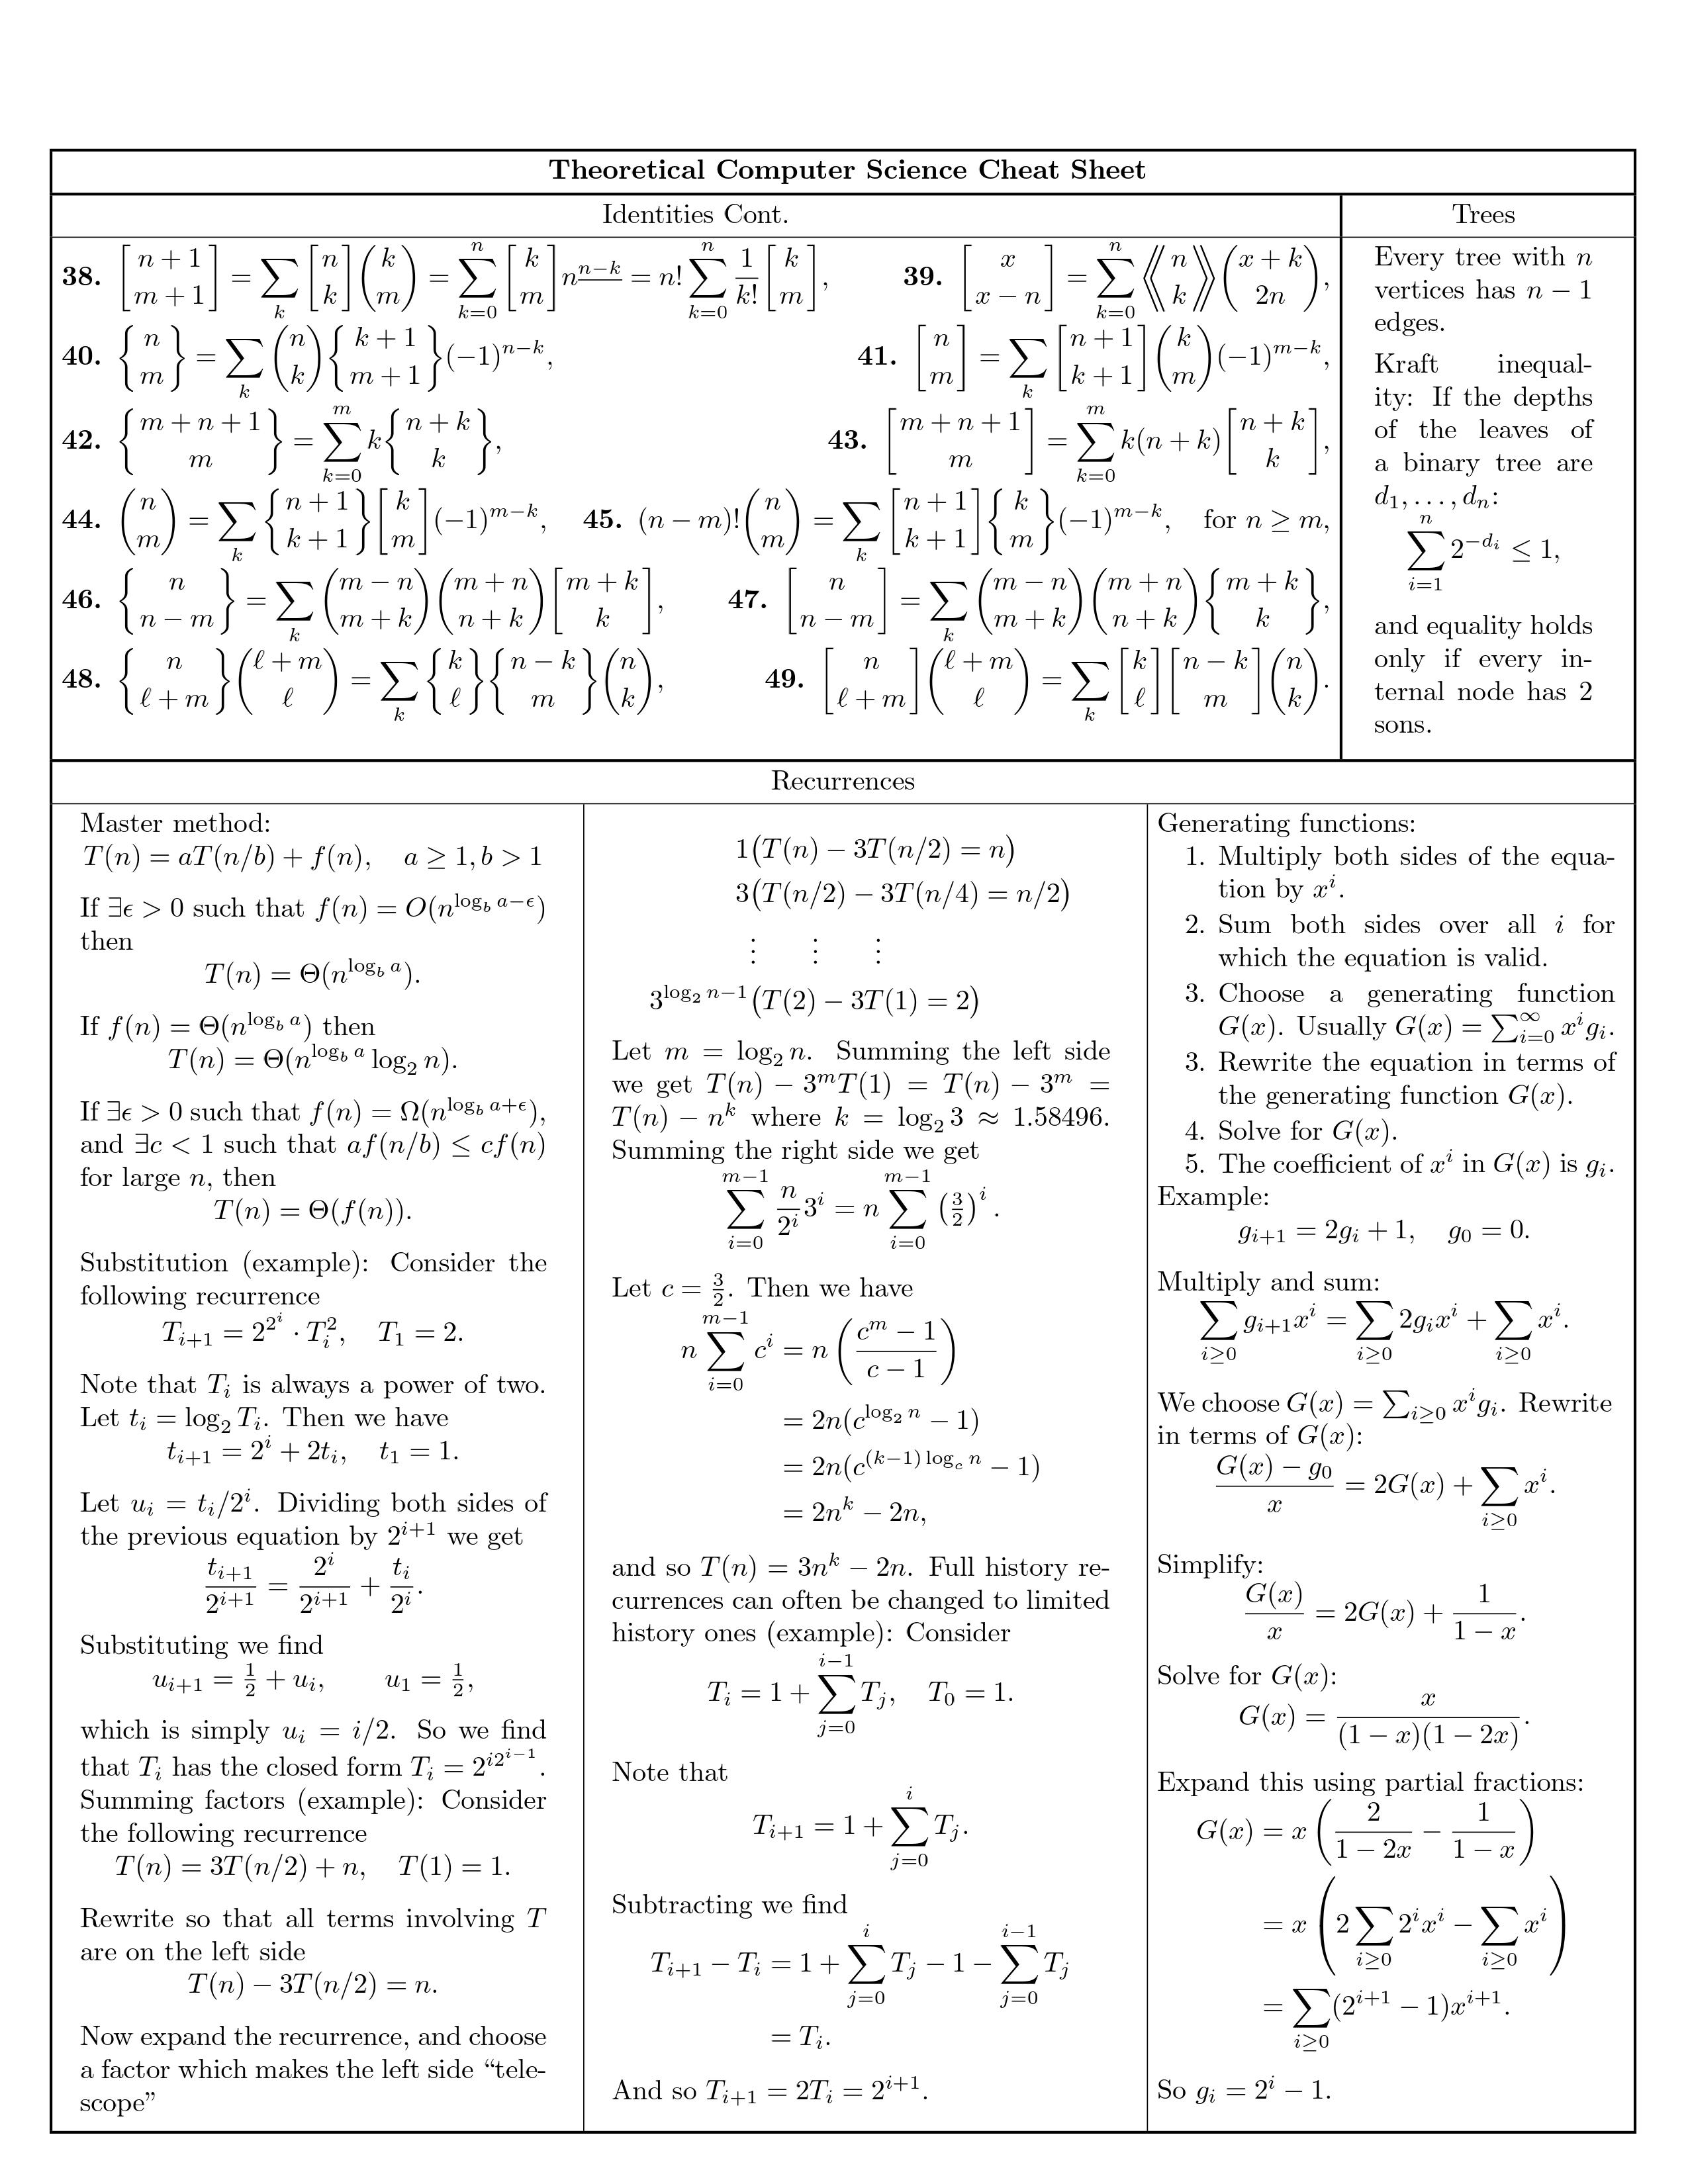
\includegraphics[trim = 6mm 2mm 0mm 10mm,clip=true,scale = 0.73]{./images/image-0002.jpg}
\newpage
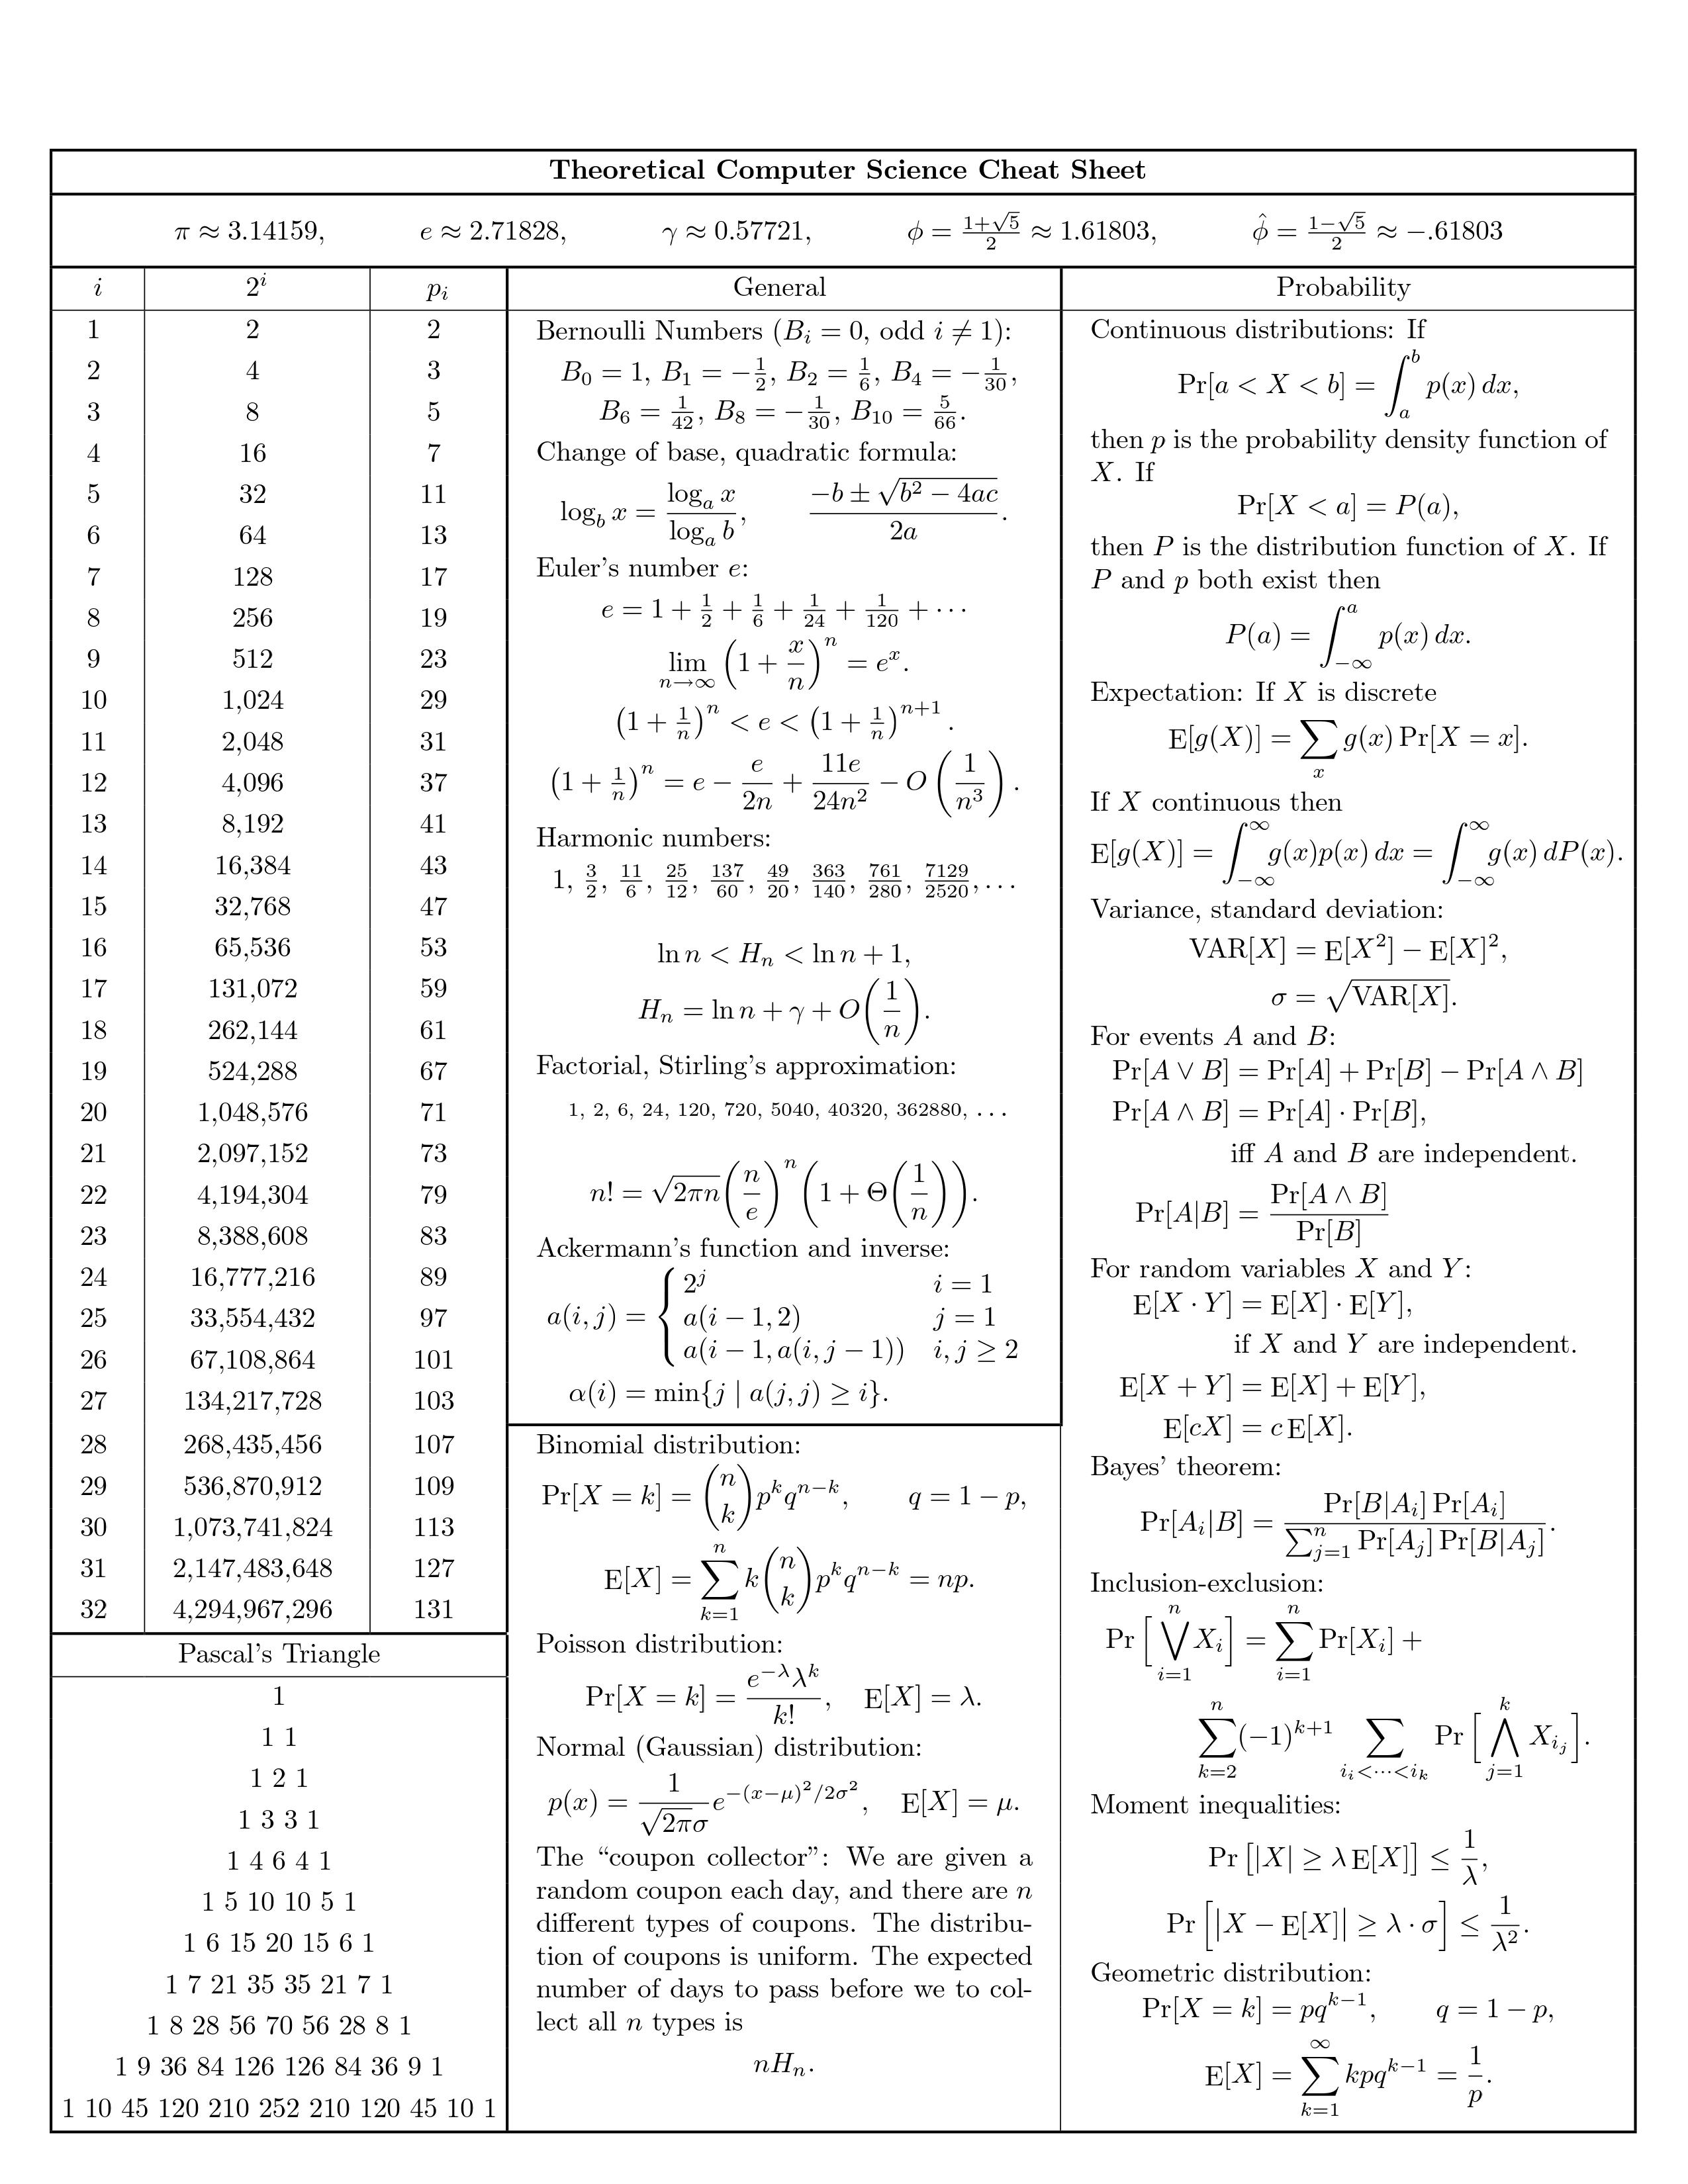
\includegraphics[trim = 6mm 2mm 0mm 10mm,clip=true,scale = 0.73]{./images/image-0003.jpg}
\newpage
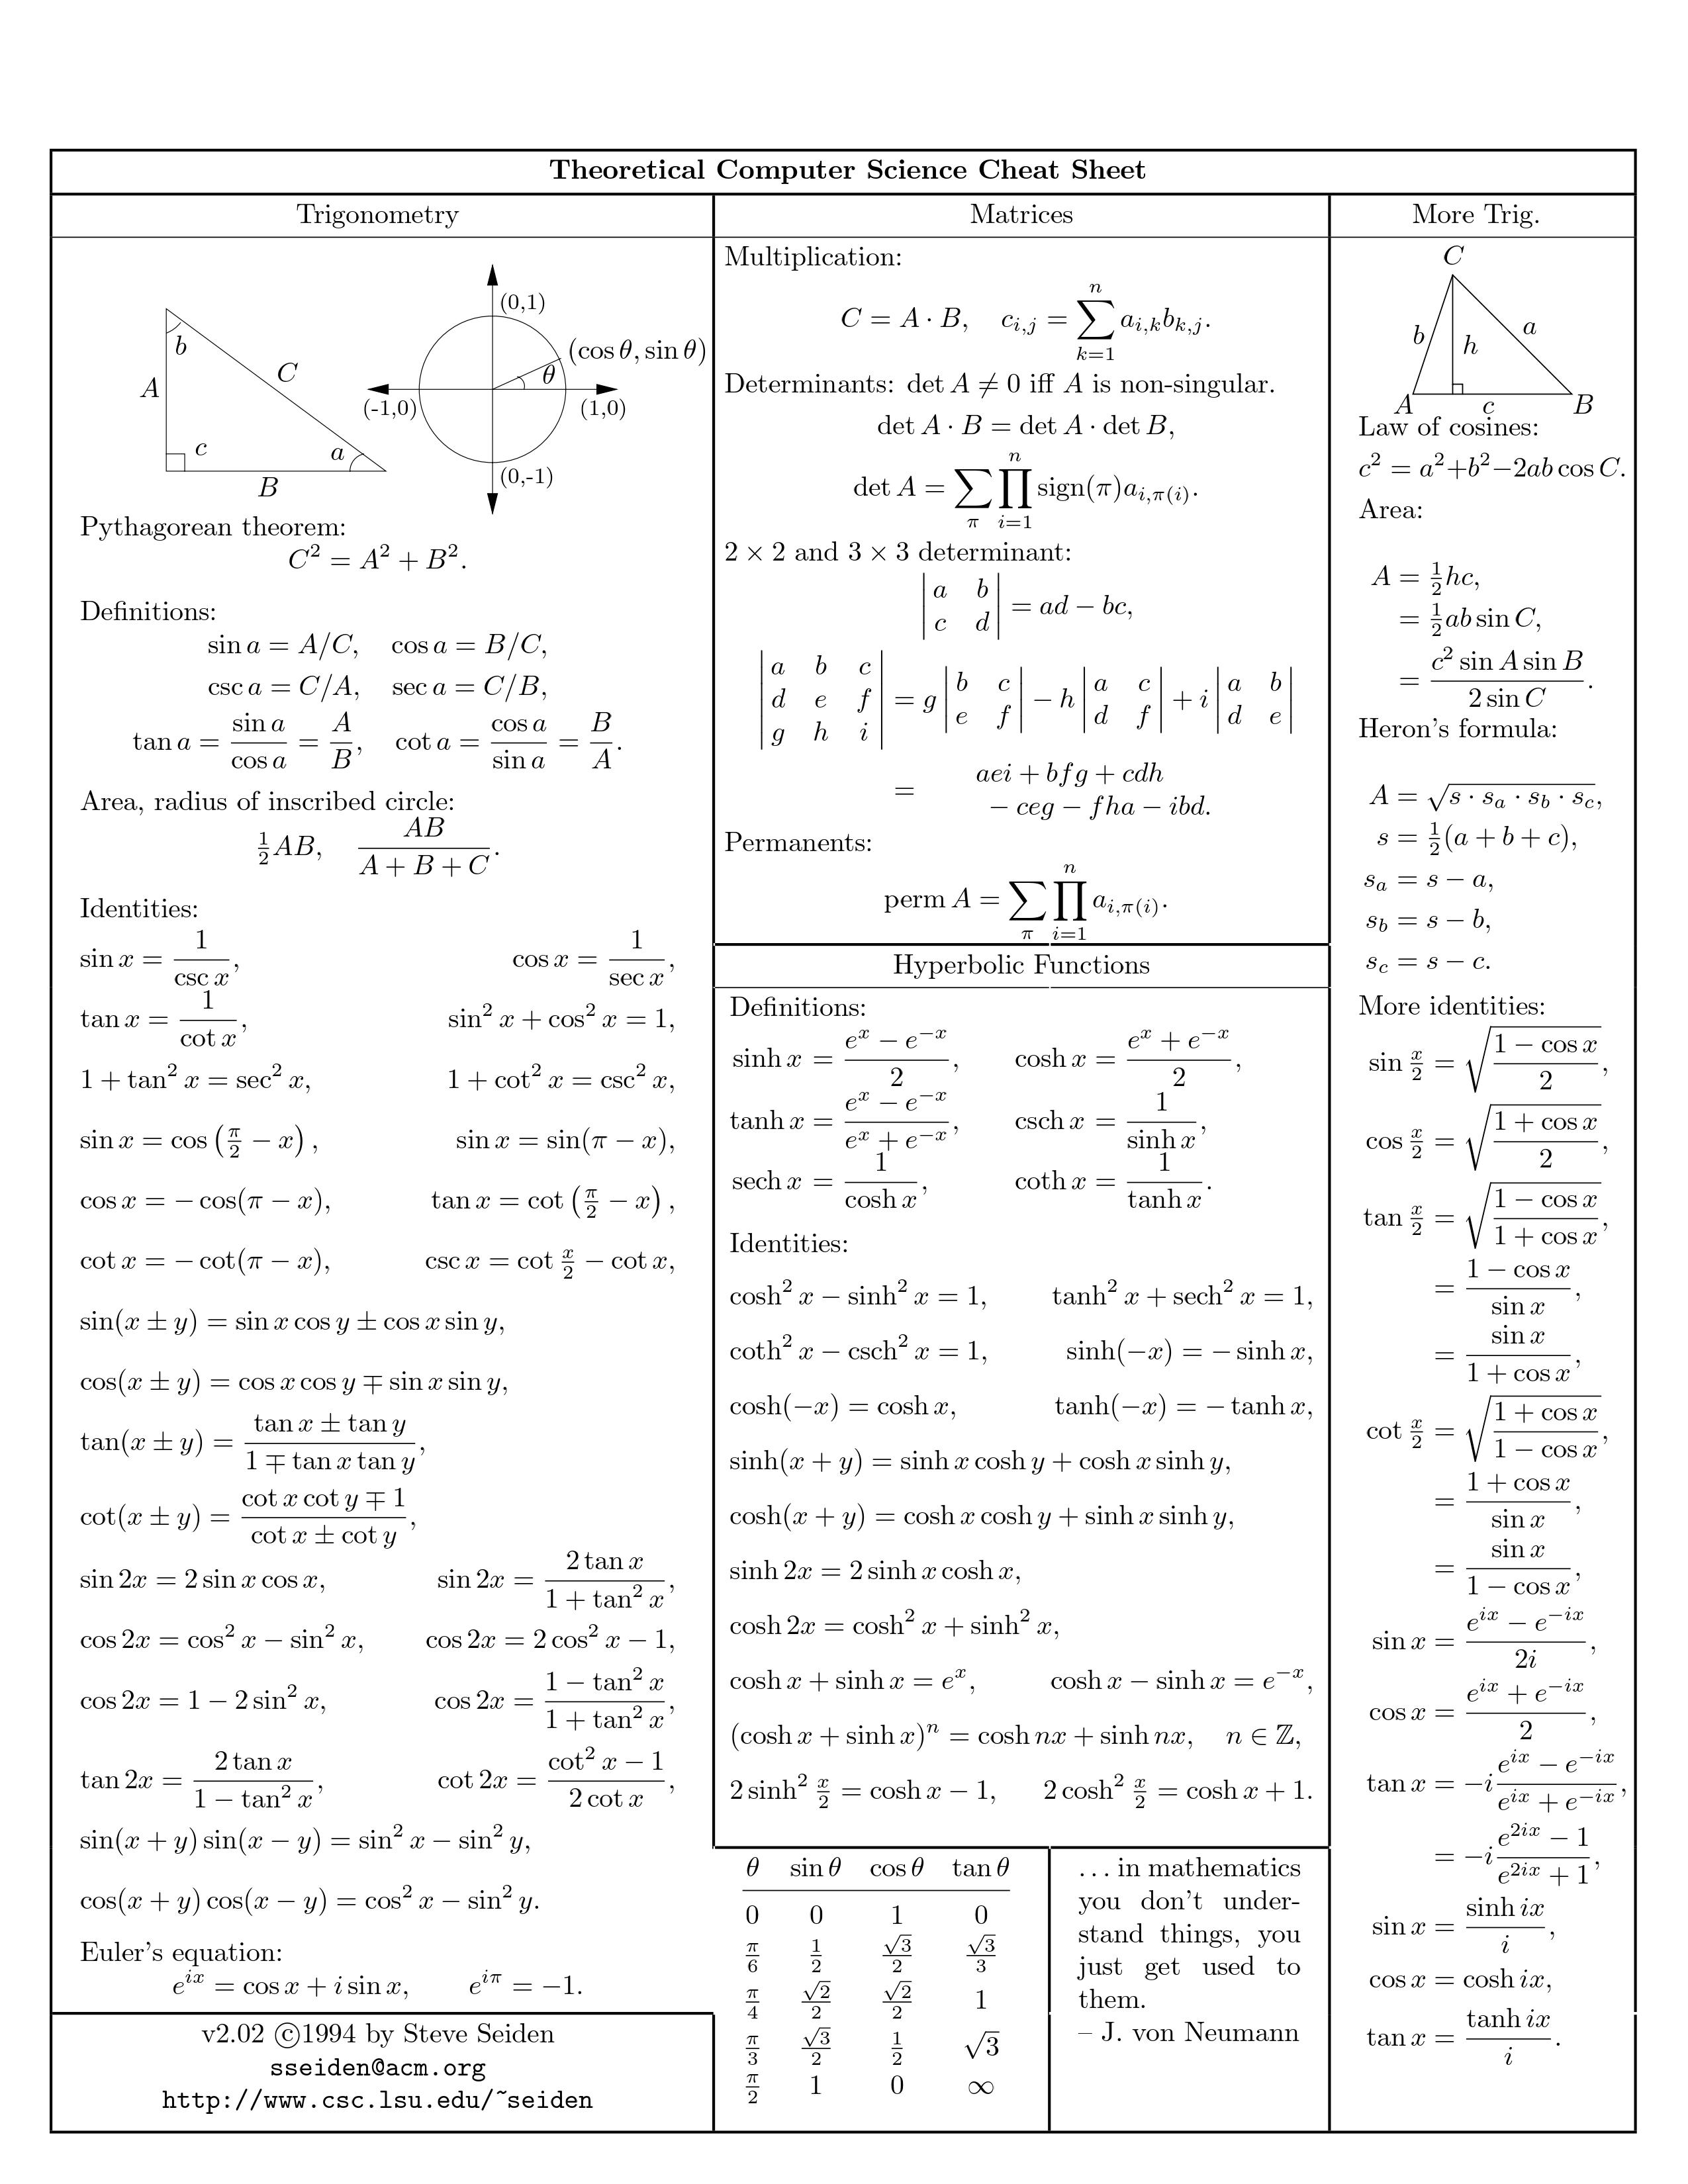
\includegraphics[trim = 6mm 2mm 0mm 10mm,clip=true,scale = 0.73]{./images/image-0004.jpg}
\newpage
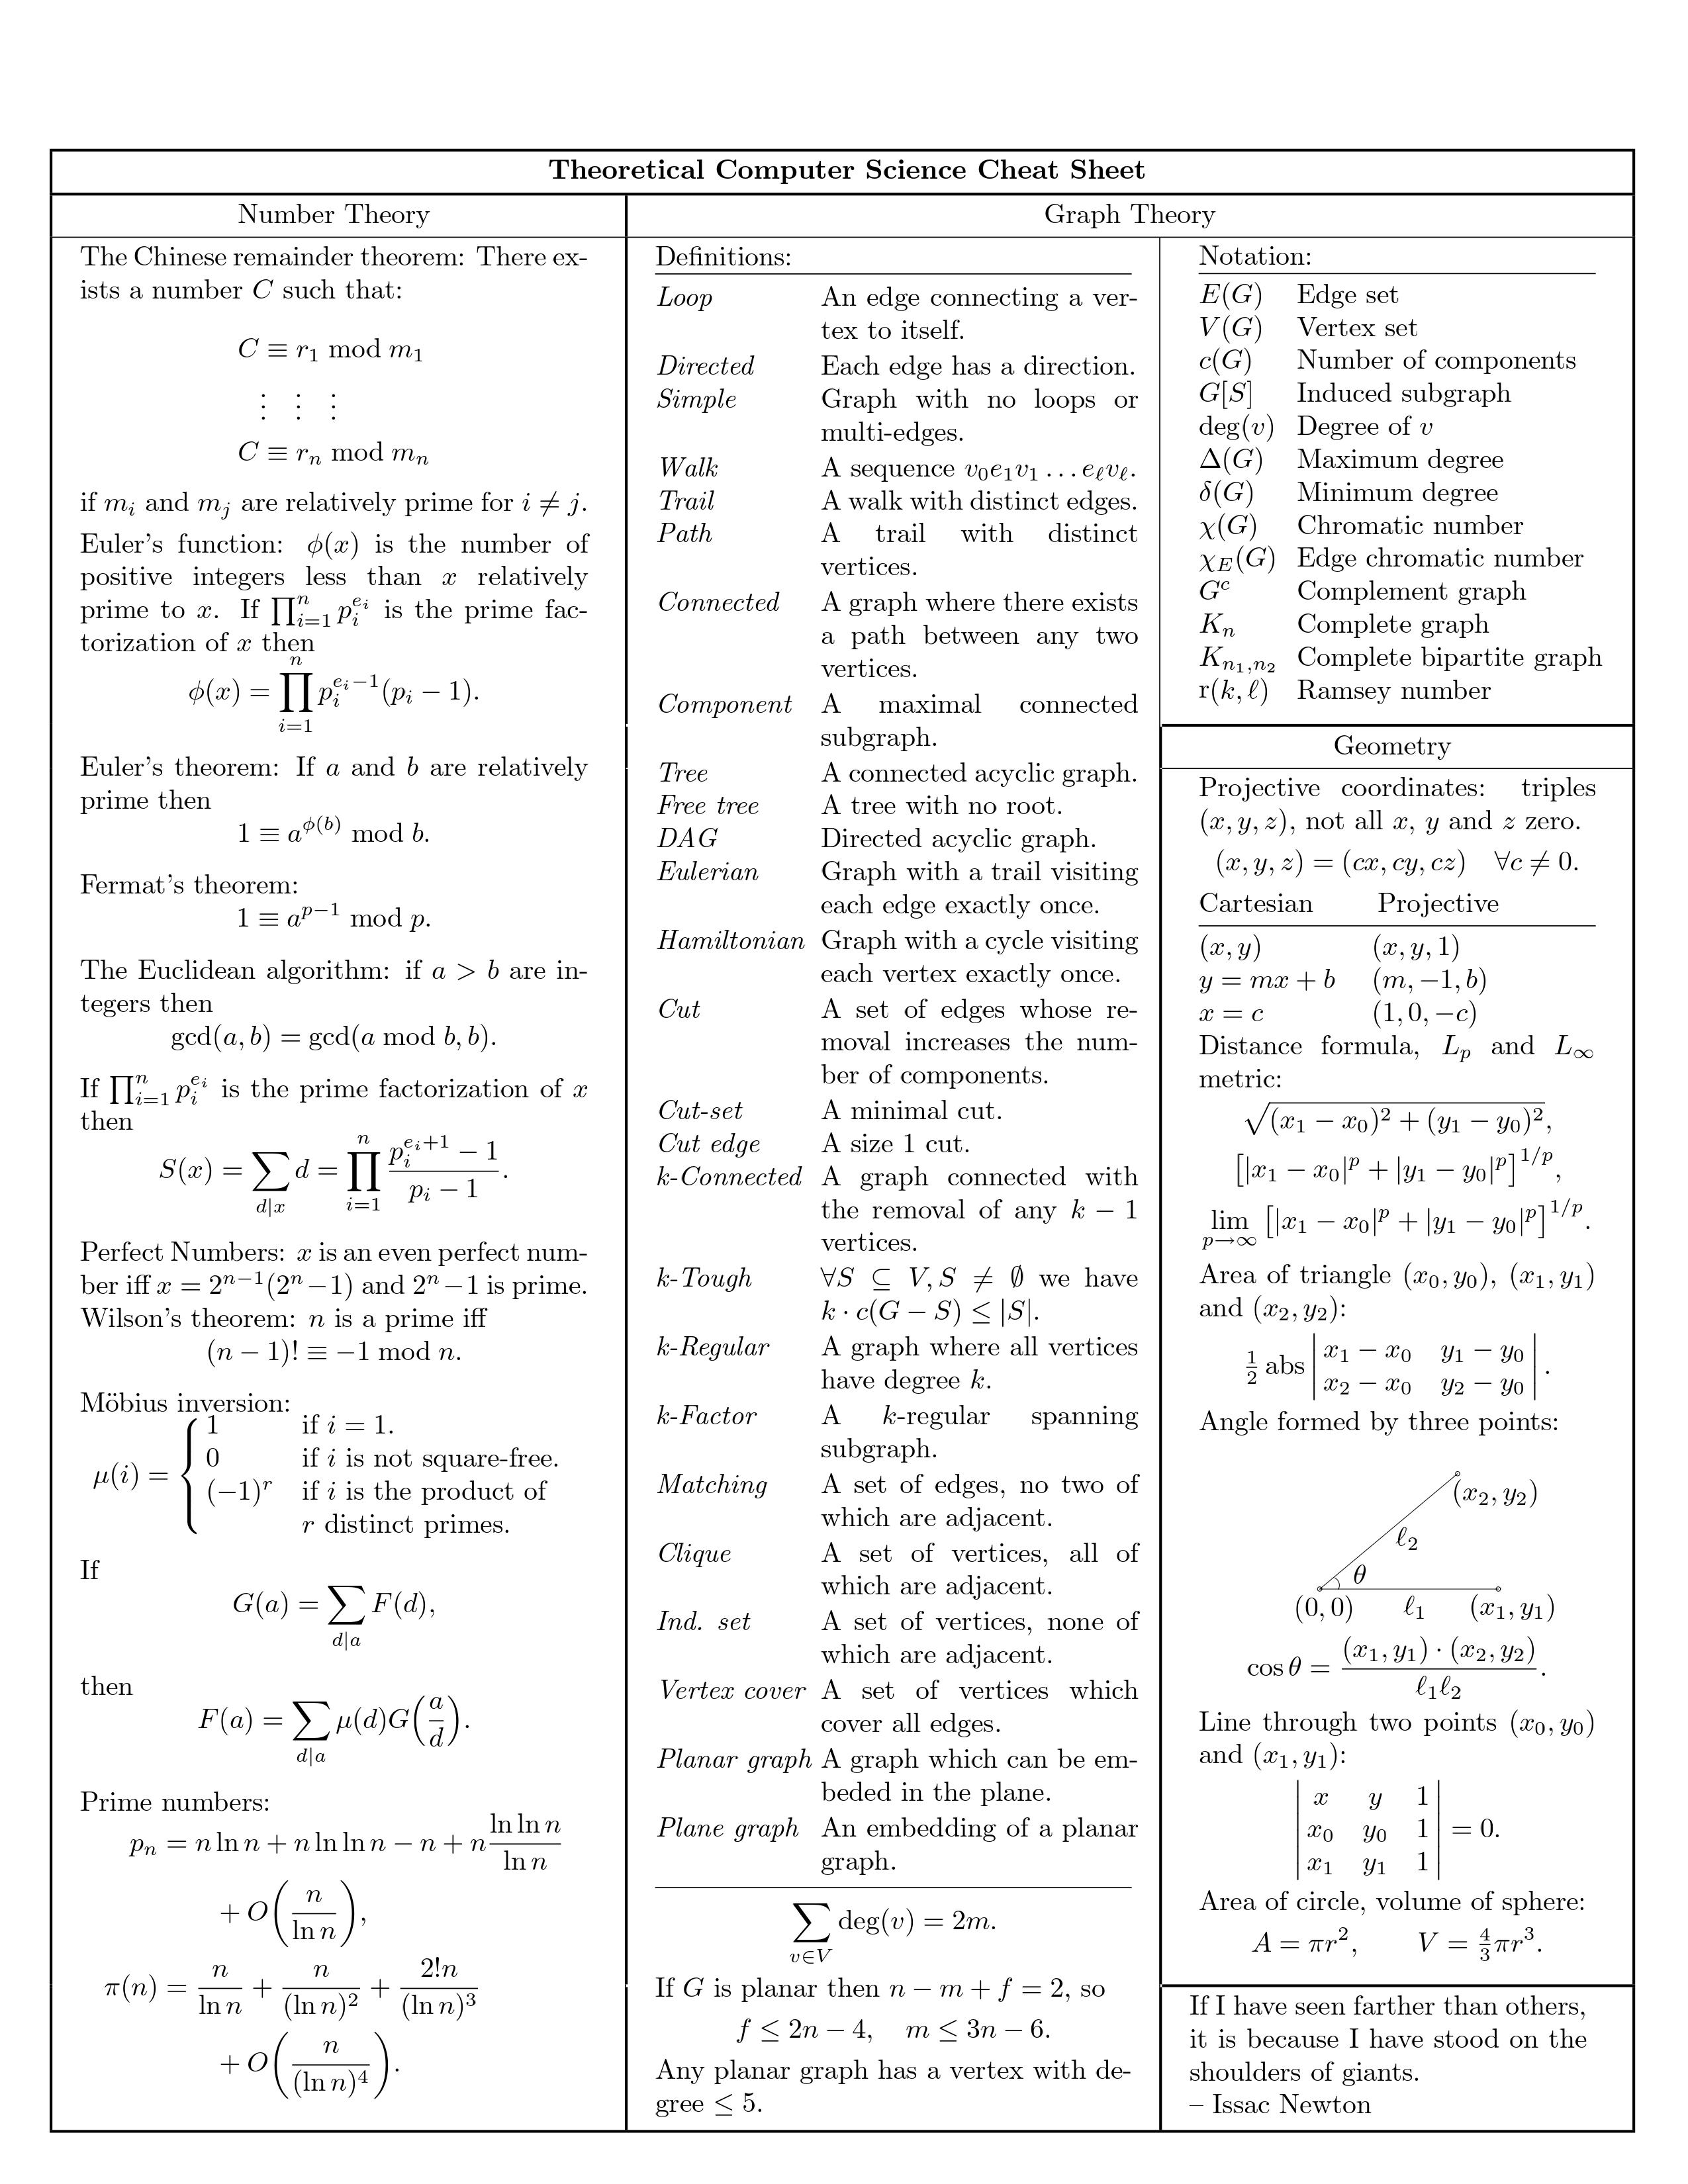
\includegraphics[trim = 6mm 2mm 0mm 10mm,clip=true,scale = 0.73]{./images/image-0005.jpg}
\newpage
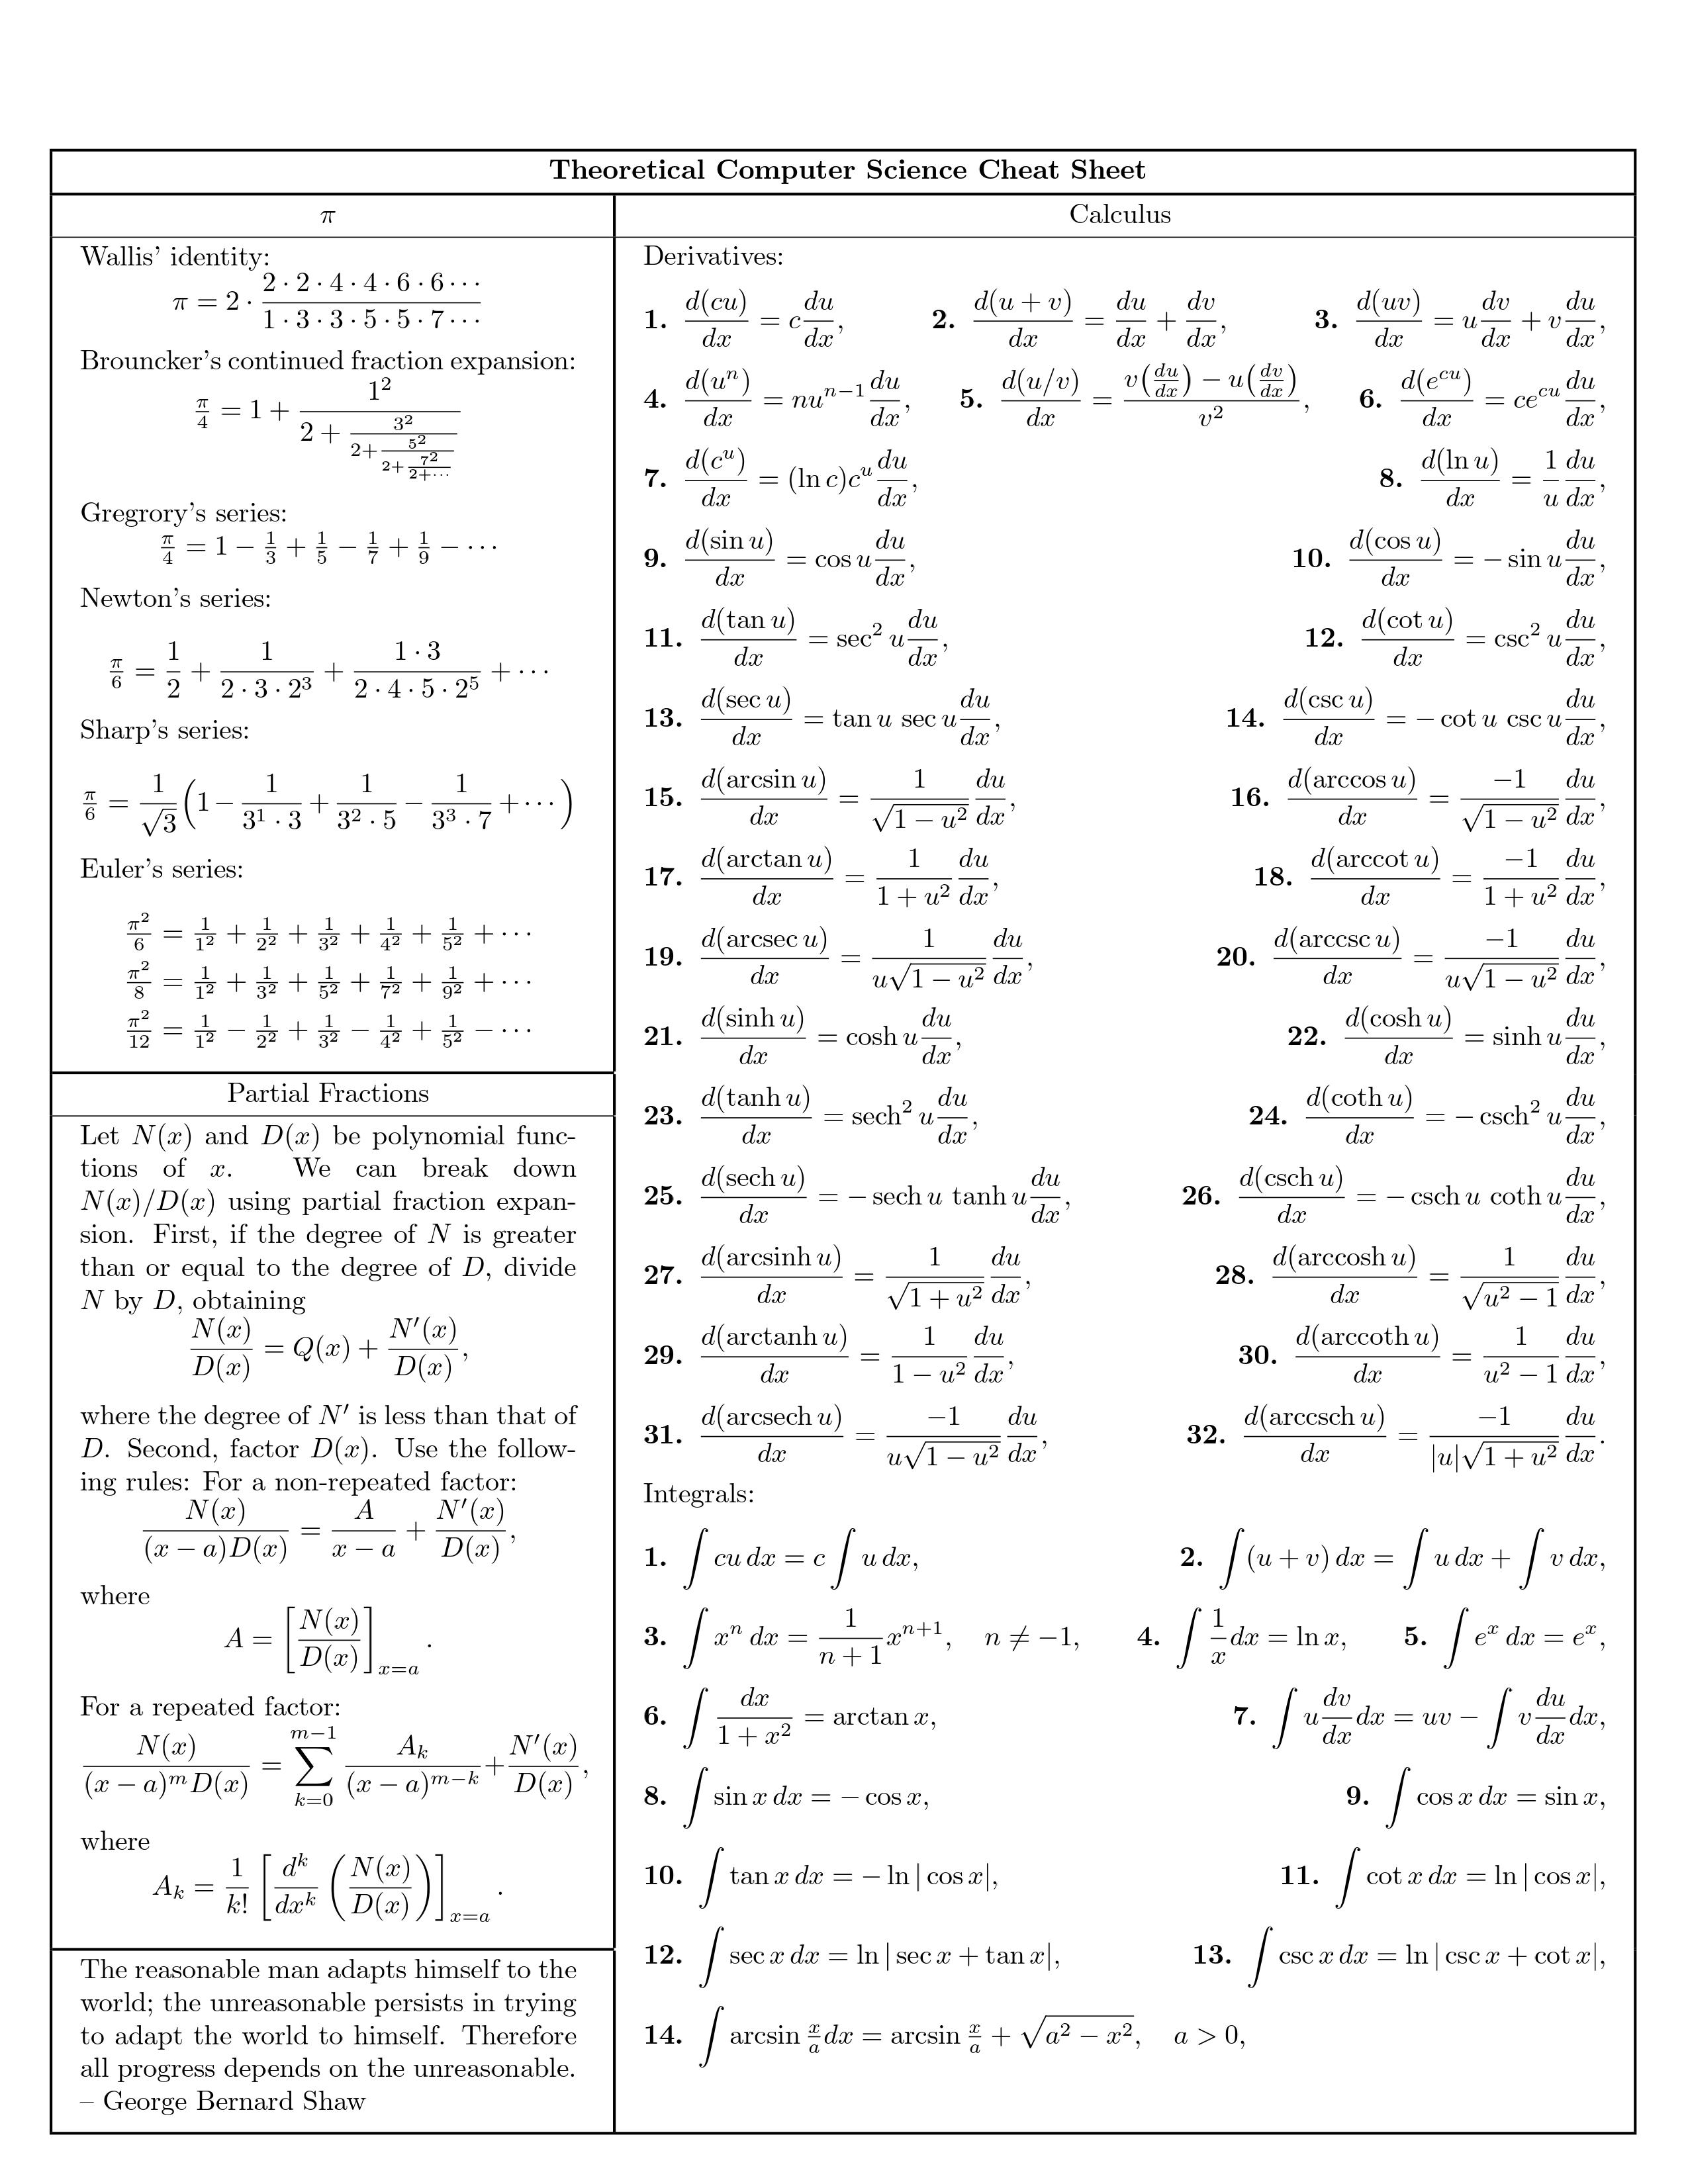
\includegraphics[trim = 6mm 2mm 0mm 10mm,clip=true,scale = 0.73]{./images/image-0006.jpg}
\newpage
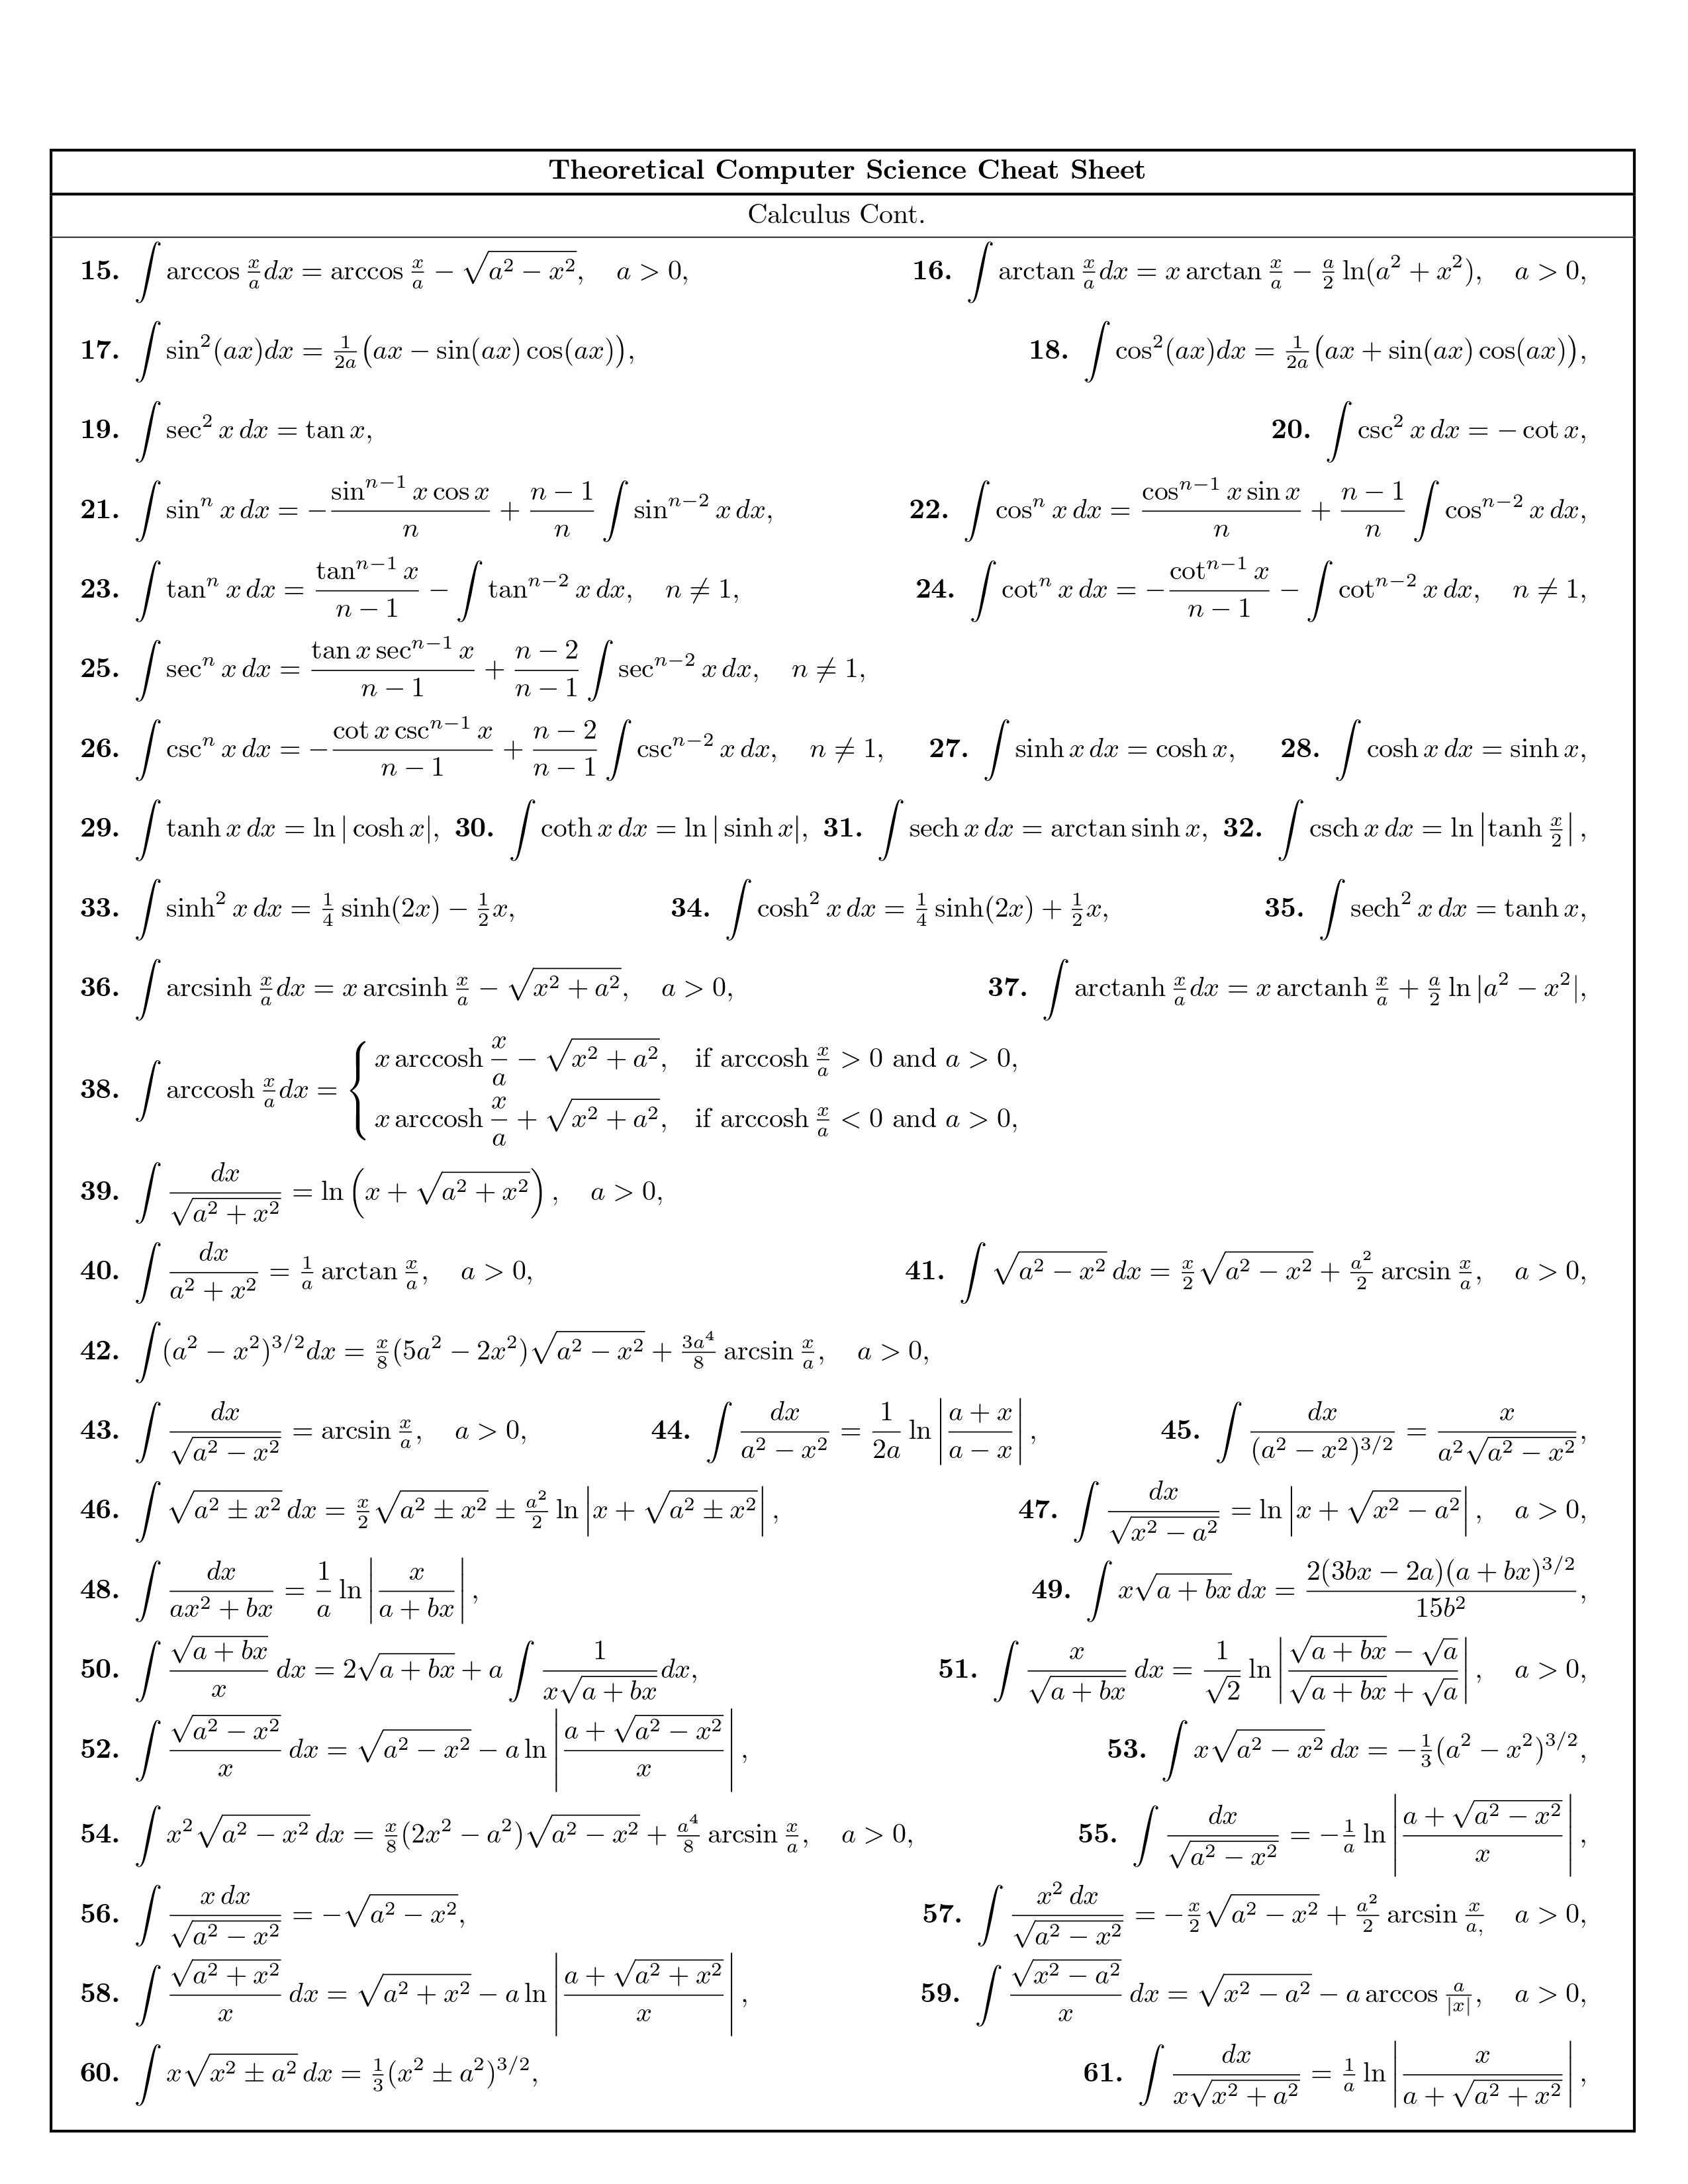
\includegraphics[trim = 6mm 2mm 0mm 10mm,clip=true,scale = 0.73]{./images/image-0007.jpg}
\newpage
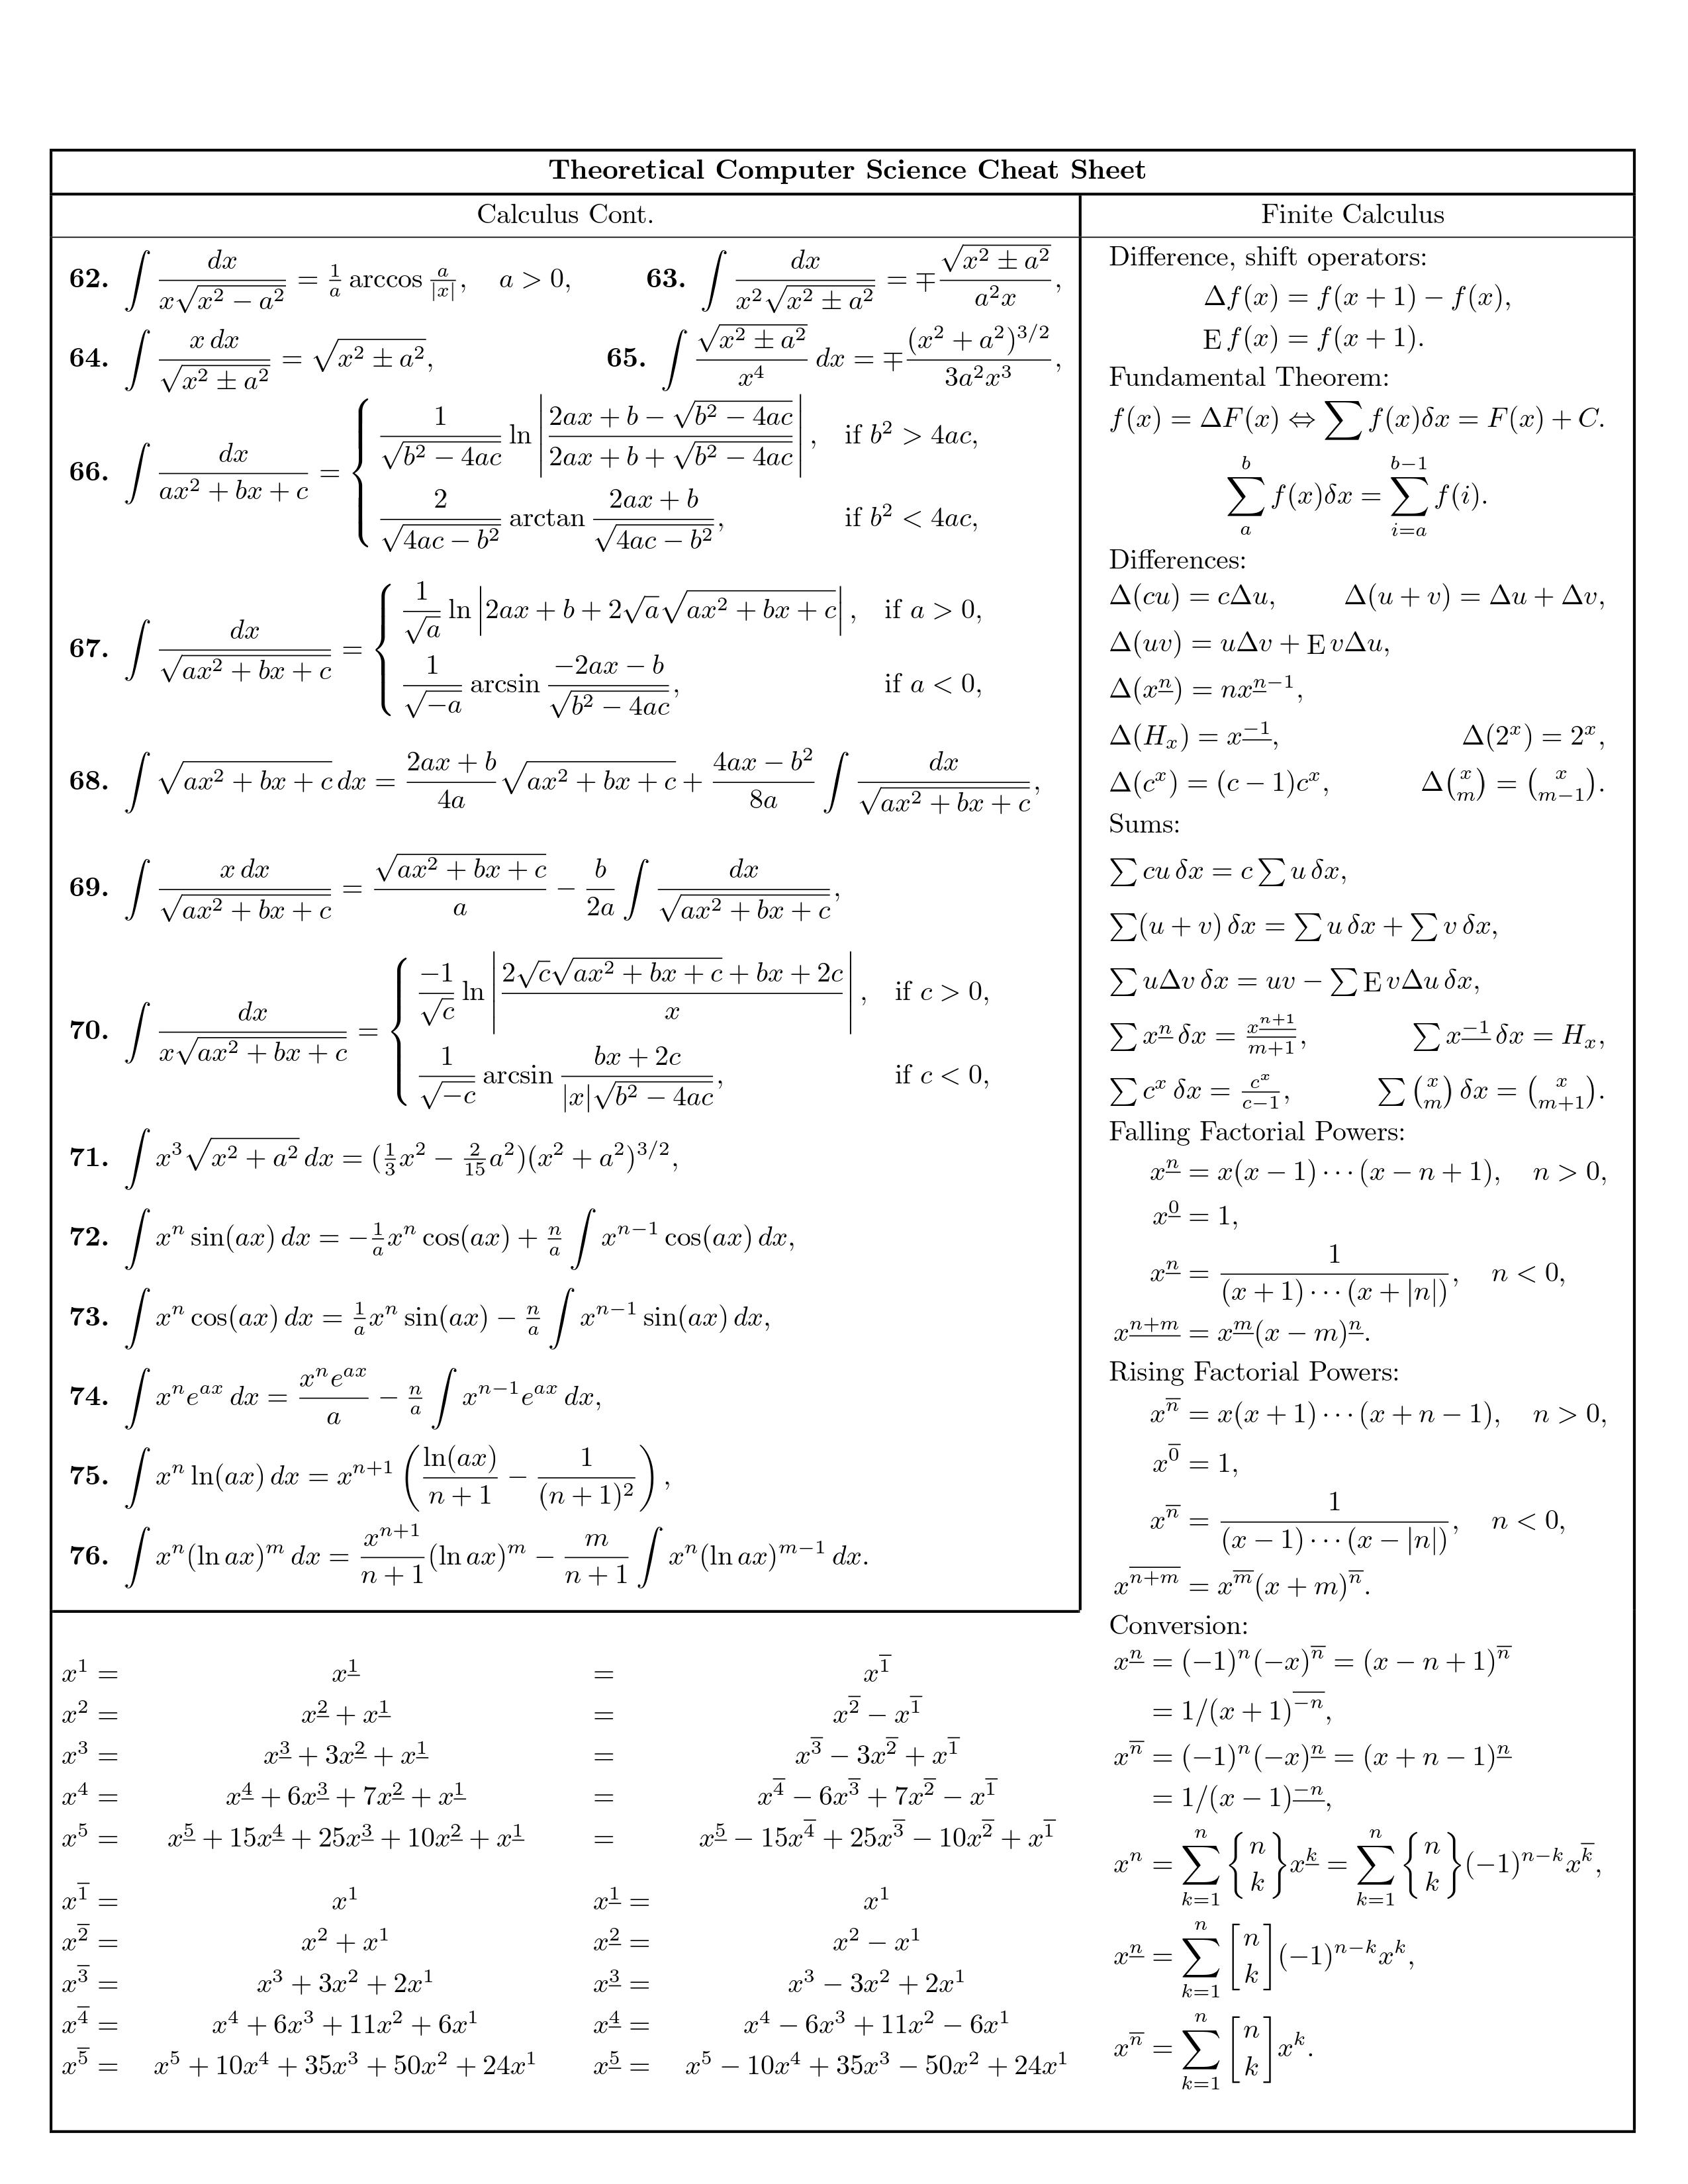
\includegraphics[trim = 6mm 2mm 0mm 10mm,clip=true,scale = 0.73]{./images/image-0008.jpg}
\newpage
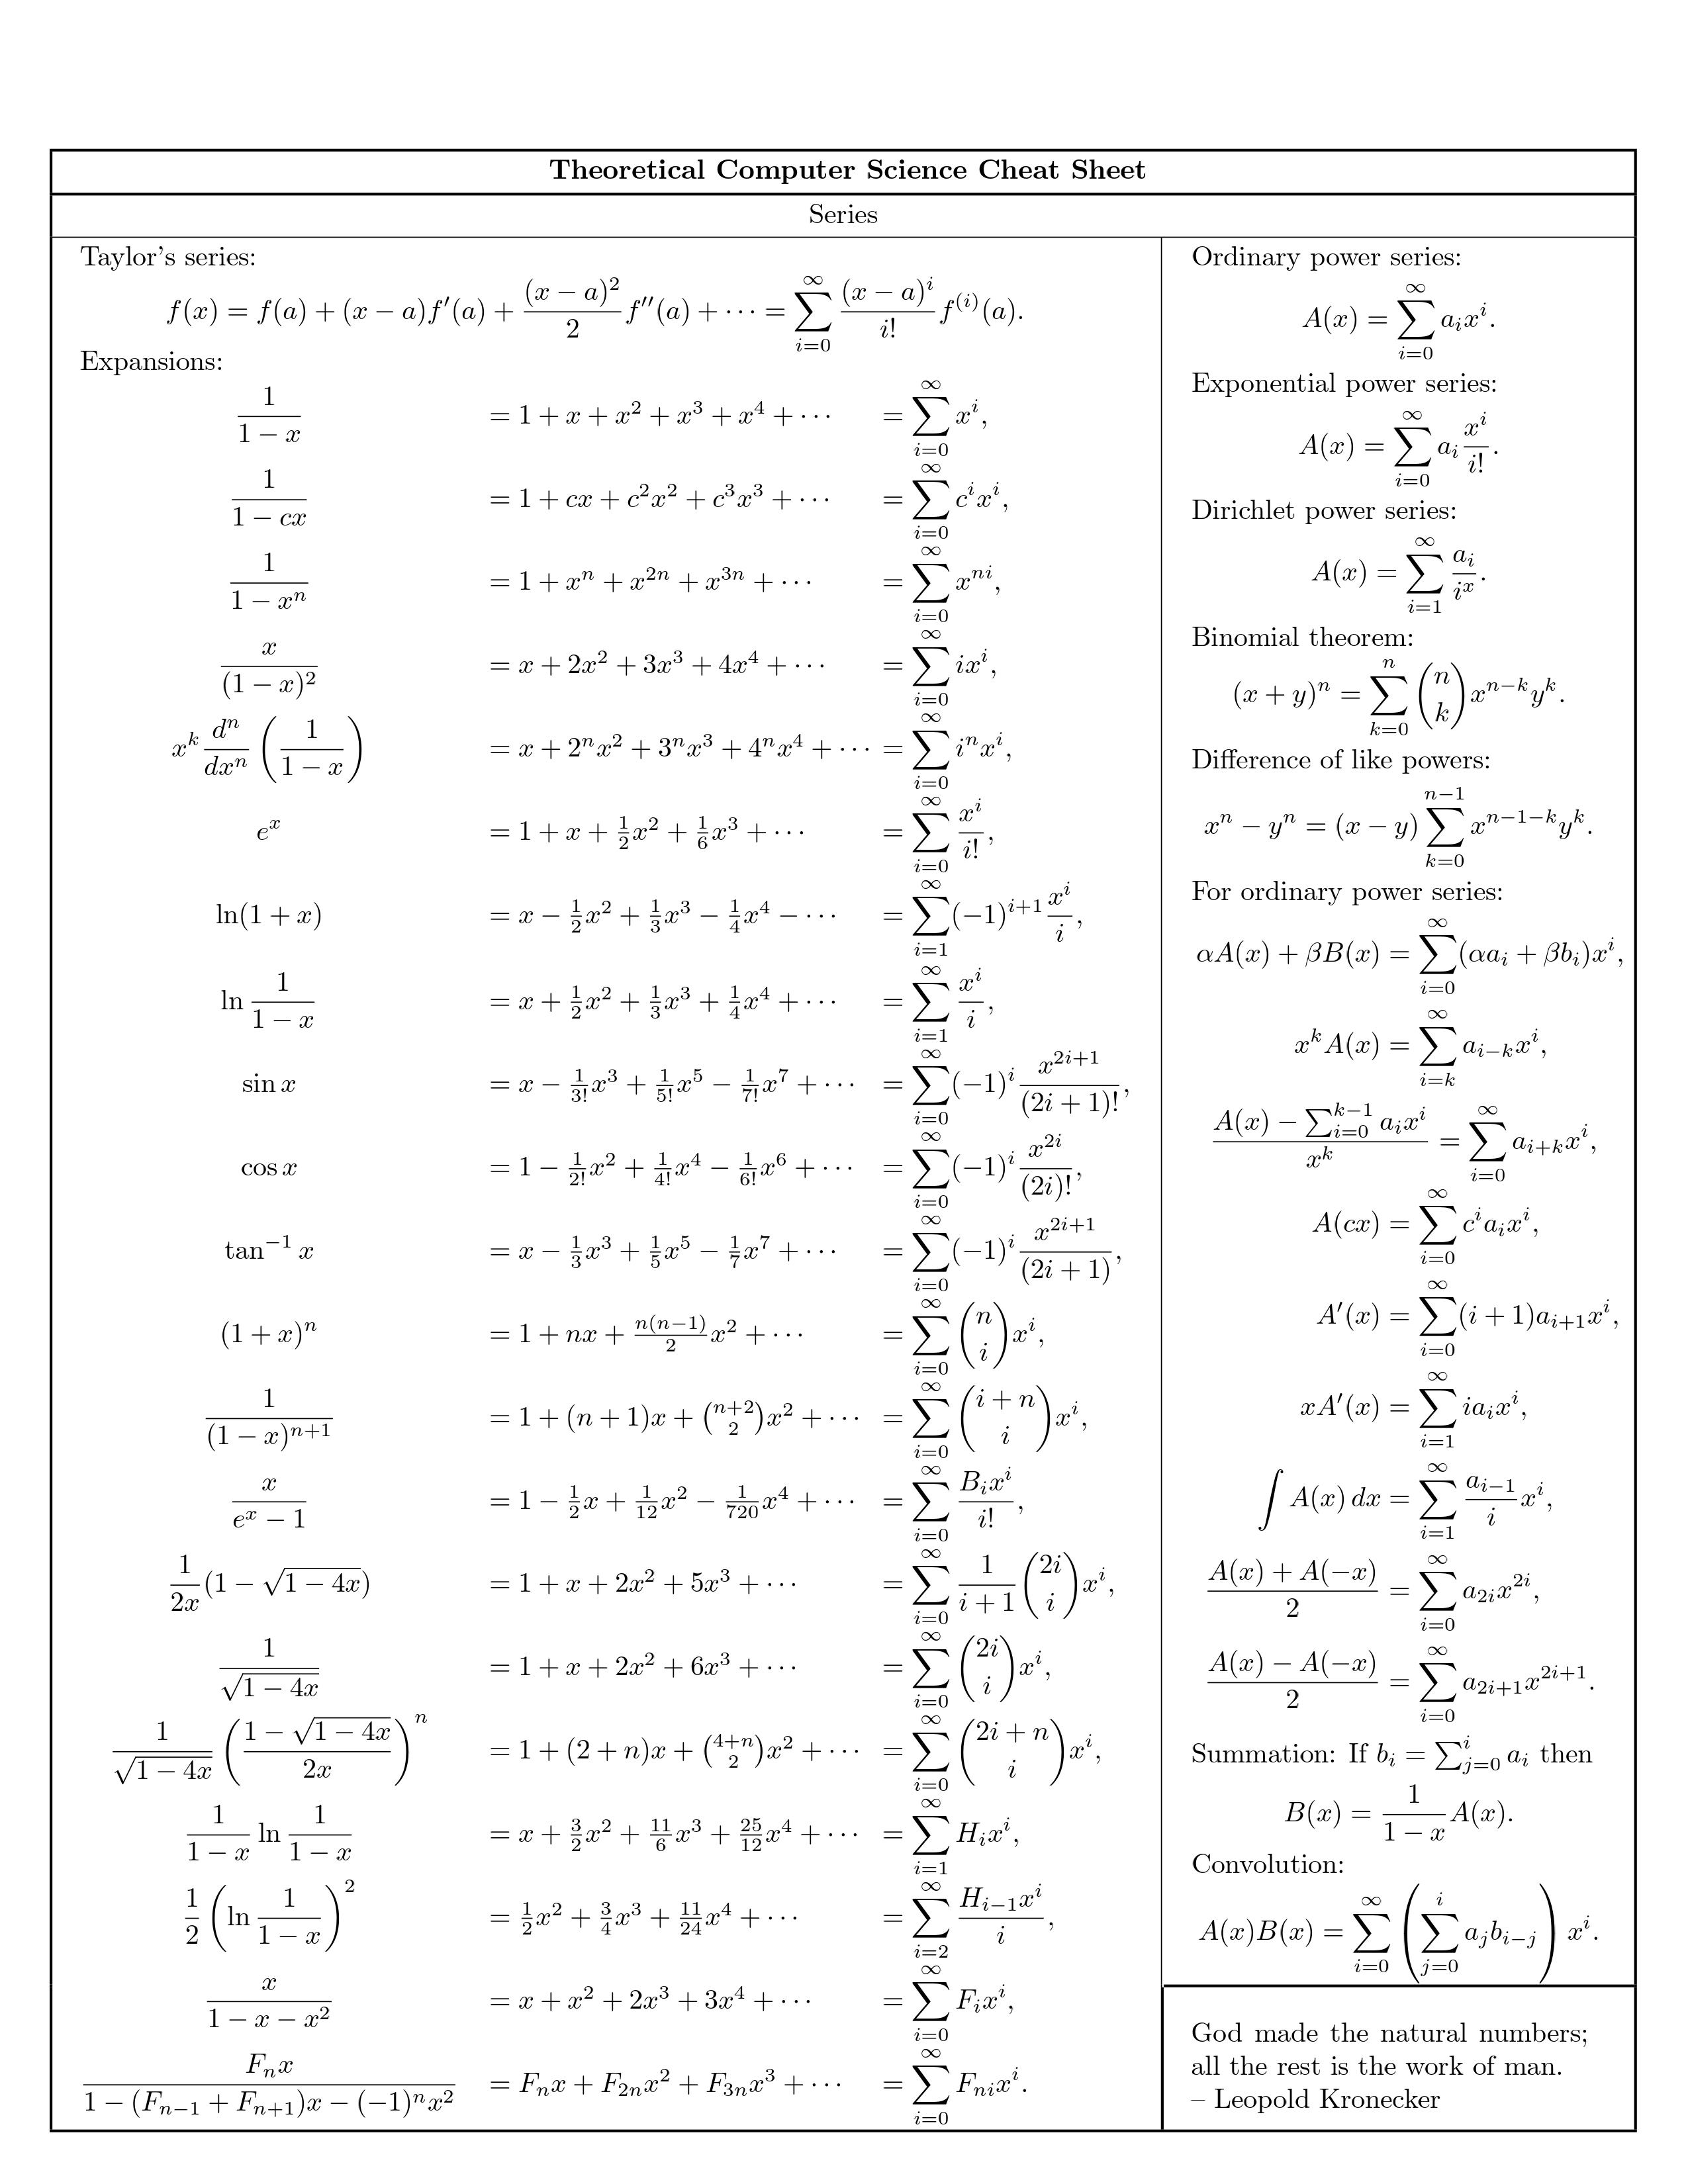
\includegraphics[trim = 6mm 2mm 0mm 10mm,clip=true,scale = 0.73]{./images/image-0009.jpg}
\newpage
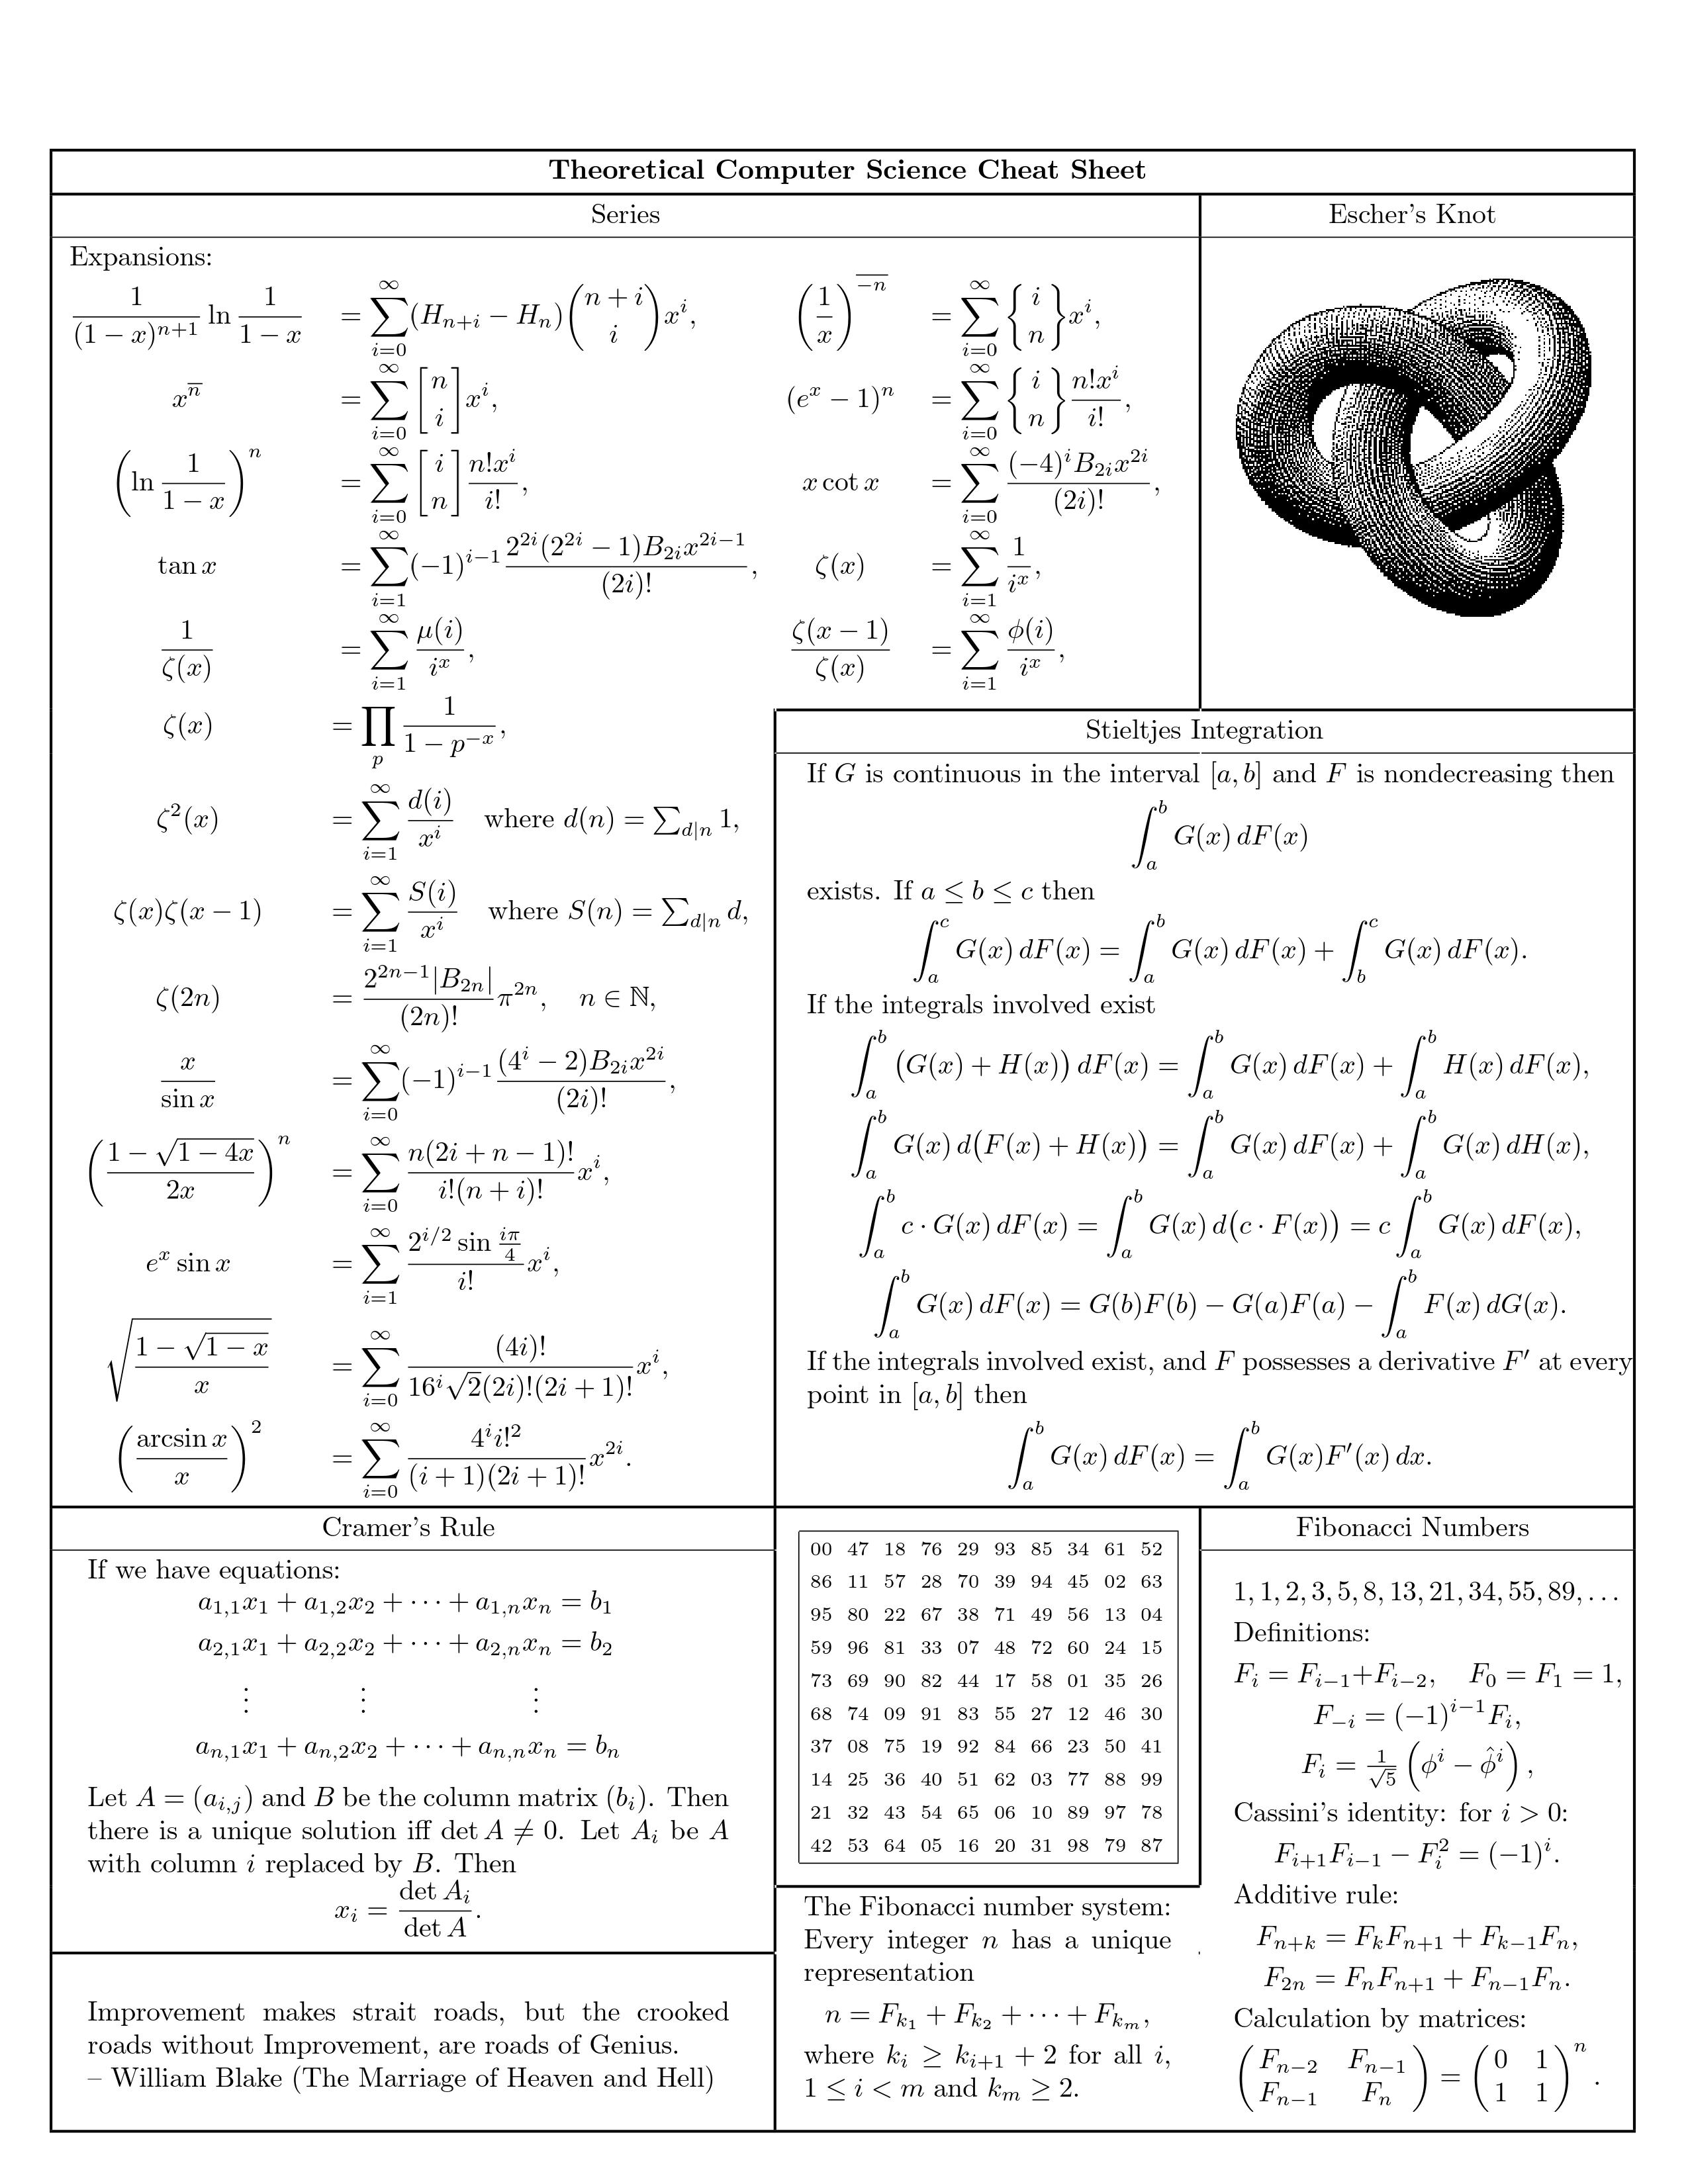
\includegraphics[trim = 6mm 2mm 0mm 10mm,clip=true,scale = 0.73]{./images/image-0010.jpg}
\end{document}
